%%%%%%%%%%%%%%%%%%%%%%%%%%%%%%%%%%%%%%%%%
% Masters/Doctoral Thesis
% LaTeX Template
% Version 2.5 (27/8/17)
%
% This template was downloaded from:
% http://www.LaTeXTemplates.com
%
% Version 2.x major modifications by:
% Vel (vel@latextemplates.com)
%
% This template is based on a template by:
% Steve Gunn (http://users.ecs.soton.ac.uk/srg/softwaretools/document/templates/)
% Sunil Patel (http://www.sunilpatel.co.uk/thesis-template/)
%
% Template license:
% CC BY-NC-SA 3.0 (http://creativecommons.org/licenses/by-nc-sa/3.0/)
%
%%%%%%%%%%%%%%%%%%%%%%%%%%%%%%%%%%%%%%%%%

%-------------------------------------------------------------------------------
%	PACKAGES AND OTHER DOCUMENT CONFIGURATIONS
%-------------------------------------------------------------------------------

\documentclass[
12pt, % The default document font size, options: 10pt, 11pt, 12pt
%oneside, % Two side (alternating margins) for binding by default, uncomment to switch to one side
spanish, % ngerman for German
onehalfspacing, % Single line spacing, alternatives: onehalfspacing or doublespacing
%draft, % Uncomment to enable draft mode (no pictures, no links, overfull hboxes indicated)
%nolistspacing, % If the document is onehalfspacing or doublespacing, uncomment this to set spacing in lists to single
%liststotoc, % Uncomment to add the list of figures/tables/etc to the table of contents
%toctotoc, % Uncomment to add the main table of contents to the table of contents
parskip, % Uncomment to add space between paragraphs
%nohyperref, % Uncomment to not load the hyperref package
headsepline, % Uncomment to get a line under the header
chapterinoneline, % Uncomment to place the chapter title next to the number on one line
%consistentlayout, % Uncomment to change the layout of the declaration, abstract and acknowledgements pages to match the default layout
]{MastersDoctoralThesis} % The class file specifying the document structure

\usepackage[utf8]{inputenc} % Required for inputting international characters
\usepackage[T1]{fontenc} % Output font encoding for international characters

\usepackage{mathpazo} % Use the Palatino font by default
\usepackage{amsmath} % More math functions

\usepackage[backend=bibtex,natbib=true]{biblatex} % Use the bibtex backend with the authoryear citation style (which resembles APA)

\addbibresource{main.bib} % The filename of the bibliography

\usepackage[autostyle=true]{csquotes} % Required to generate language-dependent quotes in the bibliography

\usepackage{listings} % Package to type bash commands

\usepackage{imakeidx} % Package to make an index of words used in the papers
\makeindex[program=makeindex,columns=2,intoc=true,options={-s index_style.ist}]

\usepackage[hidelinks]{hyperref} % Used to hide the link frames

%-------------------------------------------------------------------------------
%	MARGIN SETTINGS
%-------------------------------------------------------------------------------

\geometry{
	paper=a4paper, % Change to letterpaper for US letter
	inner=2.5cm, % Inner margin
	outer=2.5cm, % Outer margin
	top=2.5cm, % Top margin
	bottom=2.5cm, % Bottom margin
	%showframe, % Uncomment to show how the type block is set on the page
}

%-------------------------------------------------------------------------------
%	THESIS INFORMATION
%-------------------------------------------------------------------------------

\thesistitle{Aplicación para la compartición segura de ficheros} % Your thesis title, this is used in the title and abstract, print it elsewhere with \ttitle
\supervisor{Dr. Gorka Guardiola Múzquiz} % Your supervisor's name, this is used in the title page, print it elsewhere with \supname
\examiner{} % Your examiner's name, this is not currently used anywhere in the template, print it elsewhere with \examname
\degree{Grado en Ingeniería en Telemática} % Your degree name, this is used in the title page and abstract, print it elsewhere with \degreename
\author{Sergio Merino Hernández} % Your name, this is used in the title page and abstract, print it elsewhere with \authorname
\addresses{} % Your address, this is not currently used anywhere in the template, print it elsewhere with \addressname

\subject{} % Your subject area, this is not currently used anywhere in the template, print it elsewhere with \subjectname
\keywords{} % Keywords for your thesis, this is not currently used anywhere in the template, print it elsewhere with \keywordnames
\university{\href{https://www.urjc.es}{Universidad Rey Juan Carlos}} % Your university's name and URL, this is used in the title page and abstract, print it elsewhere with \univname
\department{} % Your department's name and URL, this is used in the title page and abstract, print it elsewhere with \deptname
\group{} % Your research group's name and URL, this is used in the title page, print it elsewhere with \groupname
\faculty{Escuela Técnica Superior de Ingeniería de Telecomunicación} % Your faculty's name and URL, this is used in the title page and abstract, print it elsewhere with \facname

\AtBeginDocument{
\hypersetup{pdftitle=\ttitle} % Set the PDF's title to your title
\hypersetup{pdfauthor=\authorname} % Set the PDF's author to your name
\hypersetup{pdfkeywords=\keywordnames} % Set the PDF's keywords to your keywords
}

\begin{document}

\frontmatter % Use roman page numbering style (i, ii, iii, iv...) for the pre-content pages

\pagestyle{plain} % Default to the plain heading style until the thesis style is called for the body content

%-------------------------------------------------------------------------------
%	TITLE PAGE
%-------------------------------------------------------------------------------

\begin{titlepage}
\begin{center}

\vspace*{.06\textheight}
{\scshape\LARGE \univname\par}\vspace{1.5cm} % University name
\textsc{\Large Trabajo Fin de Grado}\\[0.5cm] % Thesis type

\HRule \\[0.4cm] % Horizontal line
{\huge \bfseries \ttitle\par}\vspace{0.4cm} % Thesis title
\HRule \\[1.5cm] % Horizontal line

\begin{minipage}[t]{0.4\textwidth}
\begin{flushleft} \large
\emph{Autor:}\\
\href{https://github.com/merinhunter}{\authorname} % Author name - remove the \href bracket to remove the link
\end{flushleft}
\end{minipage}
\begin{minipage}[t]{0.4\textwidth}
\begin{flushright} \large
\emph{Tutor:} \\
\href{https://lsub.org/who/paurea/}{\supname} % Supervisor name - remove the \href bracket to remove the link
\end{flushright}
\end{minipage}\\[3cm]

\vfill

\textsc{\facname}\\\textsc{\degreename}\\[2cm] % Research group name and department name

\vfill

{\large \today}\\[4cm] % Date
%\includegraphics{Logo} % University/department logo - uncomment to place it

\vfill
\end{center}
\end{titlepage}

%-------------------------------------------------------------------------------
%	ABSTRACT PAGE
%-------------------------------------------------------------------------------

\begin{abstract}
\addchaptertocentry{\abstractname} % Add the abstract to the table of contents
La comunicación digital ha supuesto un increíble avance en la transmisión de información. Sin embargo, esto también ha desencadenado nuevas formas de robarla y falsificarla. Para solucionarlo existen multitud de algoritmos de seguridad que permiten cifrarla y firmarla, con el fin de mantener su confidencialidad, su integridad y su autenticidad.

Gracias a estos algoritmos surgen múltiples aplicaciones que permiten la comunicación preservando estas tres propiedades. Estas aplicaciones existen para la inmensa mayoría de las plataformas actuales y hacen uso de la combinación de diversos algoritmos.

En este contexto, este Trabajo de Fin de Grado se enfoca en el desarrollo de una aplicación que permita llevar a cabo comunicaciones seguras entre usuarios. Esta aplicación se va a desarrollar para el sistema operativo Android y va a hacer uso de varios algoritmos de cifrado estándar como RSA o AES.
\end{abstract}

%-------------------------------------------------------------------------------
%	ACKNOWLEDGEMENTS
%-------------------------------------------------------------------------------

%\begin{acknowledgements}
%\addchaptertocentry{\acknowledgementname} % Add the acknowledgements to the table of contents
%The acknowledgments and the people to thank go here, don't forget to include your project advisor\ldots
%\end{acknowledgements}

%-------------------------------------------------------------------------------
%	LIST OF CONTENTS/FIGURES/TABLES PAGES
%-------------------------------------------------------------------------------

\tableofcontents % Prints the main table of contents

\listoffigures % Prints the list of figures

\listoftables % Prints the list of tables

%-------------------------------------------------------------------------------
%	ABBREVIATIONS
%-------------------------------------------------------------------------------

\begin{abbreviations}{ll} % Include a list of abbreviations (a table of two columns)

\textbf{AES} & \textbf{A}dvanced \textbf{E}ncryption \textbf{S}tandard \\
\textbf{API} & \textbf{A}pplication \textbf{P}rogramming \textbf{I}nterface \\
\textbf{ART} & \textbf{A}ndroid \textbf{R}un\textbf{t}ime \\
\textbf{BC} & \textbf{B}ouncy \textbf{C}astle \\
\textbf{CBC} & \textbf{C}ipher \textbf{B}lock \textbf{C}haining \\
\textbf{CFB} & \textbf{C}ipher \textbf{F}eed\textbf{b}ack \\
\textbf{ECB} & \textbf{E}lectronic \textbf{C}ode\textbf{b}ook \\
\textbf{EOF} & \textbf{e}nd-\textbf{o}f-\textbf{f}ile \\
\textbf{HMAC} & \textbf{H}ash-based \textbf{M}essage \textbf{A}uthentication \textbf{C}ode \\
\textbf{HTTP} & \textbf{H}yper\textbf{t}ext \textbf{T}ransfer \textbf{P}rotocol \\
\textbf{IV} & \textbf{I}nitialization \textbf{V}ector \\
\textbf{JCA} & \textbf{J}ava \textbf{C}ryptography \textbf{A}rchitecture \\
\textbf{JCE} & \textbf{J}ava \textbf{C}ryptography \textbf{E}xtension \\
\textbf{JIT} & \textbf{J}ust \textbf{I}n \textbf{T}ime \\
\textbf{JVM} & \textbf{J}ava \textbf{V}irtual \textbf{M}achine \\
\textbf{MAC} & \textbf{M}essage \textbf{A}uthentication \textbf{C}ode \\
\textbf{MCD} & \textbf{M}áximo \textbf{C}omún \textbf{D}ivisor \\
\textbf{MD} & \textbf{M}essage \textbf{D}igest \\
\textbf{mcm} & \textbf{m}ínimo \textbf{c}omún \textbf{m}últiplo \\
\textbf{OFB} & \textbf{O}utput \textbf{F}eed\textbf{b}ack \\
\textbf{PSS} & \textbf{P}robabilistic \textbf{S}ignature \textbf{S}cheme \\
\textbf{QR} & \textbf{Q}uick \textbf{R}esponse \\
\textbf{RFC} & \textbf{R}equest \textbf{f}or \textbf{C}omments \\
\textbf{RSA} & \textbf{R}ivest - \textbf{S}hamir - \textbf{A}dleman \\
\textbf{SCP} & \textbf{S}ecure \textbf{C}opy \textbf{P}rotocol \\
\textbf{SHA} & \textbf{S}ecure \textbf{H}ash \textbf{A}lgorithm \\
\textbf{SSA} & \textbf{S}ignature \textbf{S}cheme with \textbf{A}ppendix \\

\end{abbreviations}

%-------------------------------------------------------------------------------
%	DEDICATION
%-------------------------------------------------------------------------------

%\dedicatory{For/Dedicated to/To my\ldots}

%-------------------------------------------------------------------------------
%	THESIS CONTENT - CHAPTERS
%-------------------------------------------------------------------------------

\mainmatter % Begin numeric (1,2,3...) page numbering

\pagestyle{thesis} % Return the page headers back to the "thesis" style

% Include the chapters of the thesis as separate files from the Chapters folder
% Uncomment the lines as you write the chapters

% Chapter 1: Introduction

\chapter{Introducción} % Main chapter title

\label{Chapter1} % For referencing this chapter elsewhere, use \ref{Chapter2}

%----------------------------------------------------------------------------------------

\section{Motivación}
Las comunicaciones seguras nacen del deseo de protegernos: de proteger con quién nos comunicamos y el qué comunicamos.

De este deseo surgen multitud de protocolos de seguridad que hoy en día usamos sin darnos cuenta. Desde una simple consulta web hasta la felicitación de Año Nuevo, nuestras comunicaciones pasan por diversas operaciones para preservar su seguridad.

Esta seguridad viene generalmente proporcionada por la confianza que depositamos en ciertas organizaciones, las cuales crean una red de confianza sobre la que se sustenta todo este sistema. Pero, ¿qué sucede si no podemos confiar en estas entidades? ¿Y si queremos ser nosotros los responsables de proporcionar la seguridad?

Con esta idea comienza la búsqueda de una herramienta que permita a los usuarios ser los artífices de su propia red de confianza, el pilar central en seguridad.

%----------------------------------------------------------------------------------------

\section{Estructura de la memoria}

% Chapter 2: Objectives

\chapter{Objetivos} % Main chapter title

\label{Chapter2}

%-------------------------------------------------------------------------------

\section{Objetivo general}

El objetivo principal es el desarrollo de una aplicación para el sistema operativo Android\index{Android}, que permita a cualquier usuario realizar una comunicación de datos de manera que se preserve la confidencialidad\index{Confidencialidad}, la integridad\index{Integridad} y la autenticación\index{Autenticación} de la información transmitida.

%-------------------------------------------------------------------------------

\section{Objetivos específicos}

Para abordar el objetivo principal del proyecto, este se ha dividido en unos objetivos más específicos:

\begin{itemize}
  \item Proporcionar un mecanismo que permita la transmisión de información entre distintos dispositivos.
  \item Desarrollar un esquema que permita cifrar y descifrar la información que se quiere transmitir.
  \item Diseñar una forma de comprobar la integridad\index{Integridad} y la autenticación\index{Autenticación} de la información.
\end{itemize}

%-------------------------------------------------------------------------------

\section{Modelo de amenaza}

En criptografía\index{Criptografía}, un modelo de amenaza (\emph{threat model}) especifica que tipo de amenazas potenciales a un sistema puede realizar un individuo (o grupo) con unos determinados recursos. Con el objetivo de proteger el sistema de estas amenazas, y únicamente estas, se diseña un determinado esquema de seguridad\index{Seguridad} para poder contrarrestarlas.

Nuestro modelo de amenaza será un atacante con conocimientos de criptoanálisis\index{Criptoanálisis} y con una capacidad de cómputo limitada, como la que puede tener un usuario normal en casa o en una oficina.

Los puntos más vulnerables de nuestro modelo son el \emph{hardware}\index{Hardware} y el \emph{software}\index{Software} sobre el que ejecuta el sistema, por lo que dejamos fuera a aquellas compañías que han trabajado en su desarrollo, como Intel, Google, Qualcomm, etc.

Debido a los recursos casi ilimitados que poseen también dejamos fuera de nuestro modelo a cualquiera de los gobiernos de las grandes potencias del mundo, como China, Corea, Rusia o Estados Unidos.

Un atacante de nuestro modelo de amenaza podría realizar los siguientes tipos de ataque:

\begin{itemize}
  \item Ataques sobre el texto cifrado\index{Cifrado} -- En este tipo de ataques el atacante dispone únicamente del texto cifrado\index{Cifrado} y no tiene acceso al texto plano. Ejemplos de este modelo son los ataques por fuerza bruta, en los que se prueba cada una de las posibles combinaciones para una clave hasta dar con la correcta.

  \item Ataque de texto plano conocido -- En este tipo de ataques se presupone que el atacante tiene acceso a un número limitado de textos planos y sus correspondientes textos cifrados. El objetivo de este tipo de ataques es el de obtener la clave de cifrado\index{Cifrado} a partir de estos pares, con el fin de poder descifrar futuras comunicaciones.

  \item Ataque de texto plano selectivo -- En este tipo de ataques el atacante puede seleccionar un número indeterminado de textos planos y obtener sus equivalentes cifrados. Con esto, un atacante puede probar distintas combinaciones y encontrar patrones sobre el texto plano para explotar alguna vulnerabilidad.

  \item Ataque de texto cifrado\index{Cifrado} selectivo -- Parecido al anterior, el atacante puede obtener un número indeterminado de textos planos a partir de sus equivalentes cifrados.

  \item Ataques sobre la clave -- En este tipo de ataques el atacante dispone de alguna información acerca de la clave de cifrado\index{Cifrado}.

  \item Ataque de intermediario (\emph{Man in the middle}) -- En este tipo de ataque el atacante retransmite o modifica la información que un usuario envía a otro, haciendo creer a ambas partes que mantienen una comunicación directa.

  \item Ataques de canal lateral (\emph{Side channel}) -- Este tipo de ataques explotan vulnerabilidades físicas del sistema informático (en lugar de basarse en debilidades del algoritmo utilizado), tales como fugas electromagnéticas o análisis de diferencias del consumo energético.
\end{itemize} \emph{\parencite{Reference20}}\\

% Chapter 3: State of the Art

\chapter{Estado del Arte} % Main chapter title

\label{Chapter3} % For referencing this chapter elsewhere, use \ref{Chapter2}

%----------------------------------------------------------------------------------------
%	SECTION 1
%----------------------------------------------------------------------------------------

\section{Main Section 1}

Lorem ipsum dolor sit amet, consectetur adipiscing elit. Aliquam ultricies lacinia euismod. Nam tempus risus in dolor rhoncus in interdum enim tincidunt. Donec vel nunc neque. In condimentum ullamcorper quam non consequat. Fusce sagittis tempor feugiat. Fusce magna erat, molestie eu convallis ut, tempus sed arcu. Quisque molestie, ante a tincidunt ullamcorper, sapien enim dignissim lacus, in semper nibh erat lobortis purus. Integer dapibus ligula ac risus convallis pellentesque.

%-----------------------------------
%	SUBSECTION 1
%-----------------------------------
\subsection{Subsection 1}

Nunc posuere quam at lectus tristique eu ultrices augue venenatis. Vestibulum ante ipsum primis in faucibus orci luctus et ultrices posuere cubilia Curae; Aliquam erat volutpat. Vivamus sodales tortor eget quam adipiscing in vulputate ante ullamcorper. Sed eros ante, lacinia et sollicitudin et, aliquam sit amet augue. In hac habitasse platea dictumst.

%-----------------------------------
%	SUBSECTION 2
%-----------------------------------

\subsection{Subsection 2}
Morbi rutrum odio eget arcu adipiscing sodales. Aenean et purus a est pulvinar pellentesque. Cras in elit neque, quis varius elit. Phasellus fringilla, nibh eu tempus venenatis, dolor elit posuere quam, quis adipiscing urna leo nec orci. Sed nec nulla auctor odio aliquet consequat. Ut nec nulla in ante ullamcorper aliquam at sed dolor. Phasellus fermentum magna in augue gravida cursus. Cras sed pretium lorem. Pellentesque eget ornare odio. Proin accumsan, massa viverra cursus pharetra, ipsum nisi lobortis velit, a malesuada dolor lorem eu neque.

%----------------------------------------------------------------------------------------
%	SECTION 2
%----------------------------------------------------------------------------------------

\section{Main Section 2}

Sed ullamcorper quam eu nisl interdum at interdum enim egestas. Aliquam placerat justo sed lectus lobortis ut porta nisl porttitor. Vestibulum mi dolor, lacinia molestie gravida at, tempus vitae ligula. Donec eget quam sapien, in viverra eros. Donec pellentesque justo a massa fringilla non vestibulum metus vestibulum. Vestibulum in orci quis felis tempor lacinia. Vivamus ornare ultrices facilisis. Ut hendrerit volutpat vulputate. Morbi condimentum venenatis augue, id porta ipsum vulputate in. Curabitur luctus tempus justo. Vestibulum risus lectus, adipiscing nec condimentum quis, condimentum nec nisl. Aliquam dictum sagittis velit sed iaculis. Morbi tristique augue sit amet nulla pulvinar id facilisis ligula mollis. Nam elit libero, tincidunt ut aliquam at, molestie in quam. Aenean rhoncus vehicula hendrerit.

% Chapter 4: Design and Implementation

\chapter{Diseño e implementación} % Main chapter title

\label{Chapter4} % Reference

%-------------------------------------------------------------------------------

\section{Arquitectura de seguridad}

Para entender la arquitectura de seguridad de la aplicación, es importante distinguir entre las siguientes propiedades de la seguridad de la información: confidencialidad, integridad y autenticación.

\subsection{Confidencialidad}

Para el cifrado de la información se utiliza criptografía de clave simétrica, ya que ofrece una mayor velocidad de cifrado frente a otros modelos. Debido a que puede funcionar tanto sobre \emph{hardware} como sobre \emph{software}, a que es un estándar del cifrado simétrico y a que no tiene debilidades conocidas, AES es el algoritmo de cifrado simétrico que se utiliza en esta aplicación. (Véase~\ref{AES})

De entre todos los tamaños de clave disponibles se ha optado por el de 128 \emph{bits}, ya que ofrece un nivel de seguridad adecuado para la aplicación. Además, un nivel superior habría supuesto una mayor carga computacional.

Igualmente, es necesario cifrar la clave simétrica utilizada. Para ello se utiliza un sistema de cifrado asimétrico para proteger la clave. Debido otra vez a que es un estándar, se utiliza RSA como algoritmo de cifrado asimétrico. (Véase~\ref{RSA})

Ya que el número de operaciones de cifrado asimétrico es menor que el del simétrico, se utiliza el tamaño máximo para una clave RSA: 4096 \emph{bits}.

\subsection{Integridad}

También es importante que el mensaje permanezca íntegro. Para ello se incluye junto con el mensaje una HMAC. (Véase~\ref{HMAC})

De entre algunos algoritmos de codificación se ha decidido utilizar PSS. Este algoritmo, entre otras cosas, combina el uso de una \emph{salt} con un resumen \emph{hash}, lo cual lo hace más robusto frente a determinados ataques enfocados en la obtención del mensaje original a partir de su resumen. (Véase~\ref{PSS})

\subsection{Autenticación}

El destinatario tiene que poder autenticar al autor del mensaje. Para lograrlo se incluye junto al mensaje una HMAC. (Véase~\ref{HMAC})

Se utiliza como algoritmo de firma RSASSA-PSS, ya que combina los algoritmos utilizados para preservar la confidencialidad y la integridad. Este algoritmo genera un mensaje codificado a partir del resumen del mensaje original, utilizando para ello PSS, y luego firma (cifra) este mensaje usando RSA. (Véase~\ref{RSASSA-PSS})

Para proporcionar confidencialidad a la firma, esta va cifrada usando la clave pública del destinatario, de forma que nadie más pueda acceder a su contenido.

%-------------------------------------------------------------------------------

\section{Arquitectura del software}

\label{Chapter4.2}

El objetivo de este \emph{software} es proporcionar una herramienta que permita a los usuarios mantener comunicaciones con otros usuarios preservando las tres propiedades de la seguridad comentadas en el punto anterior. Para ello, se ha llevado a cabo el desarrollo de varios prototipos:

\begin{itemize}
  \item El primer prototipo sienta las bases de la arquitectura de orientación a objetos que utiliza la aplicación. Posee un esquema que recibe un fichero y lo divide en varios fragmentos de un tamaño dado, almacenando estos fragmentos en estructuras de datos. También puede recomponer el fichero original a partir de los fragmentos.

  \item El segundo prototipo realiza las mismas tareas que el anterior, y además añade confidencialidad a los fragmentos mediante un sistema de cifrado simétrico.

  \item El tercer prototipo realiza las mismas tareas que el anterior, y además añade el uso de RSA para cifrar claves simétricas y proporcionar integridad y autenticación a los fragmentos.

  \item El cuarto prototipo realiza las mismas tareas que el anterior, ahora como una aplicación en Android. Se añade una interfaz gráfica y hace uso de algunas herramientas que posee Android para el almacenamiento de claves.
\end{itemize}

\subsection{Shatter I}

El primer prototipo de la aplicación está desarrollado enteramente en Java, usando para ello el entorno de desarrollo Eclipse. Esta primera versión busca poder dividir un fichero en varios fragmentos de un tamaño dado, y luego poder recomponerlo. Para ello se han implementado algunas clases para almacenar los datos de los fragmentos:

\begin{figure}[!htb]
  \centering
  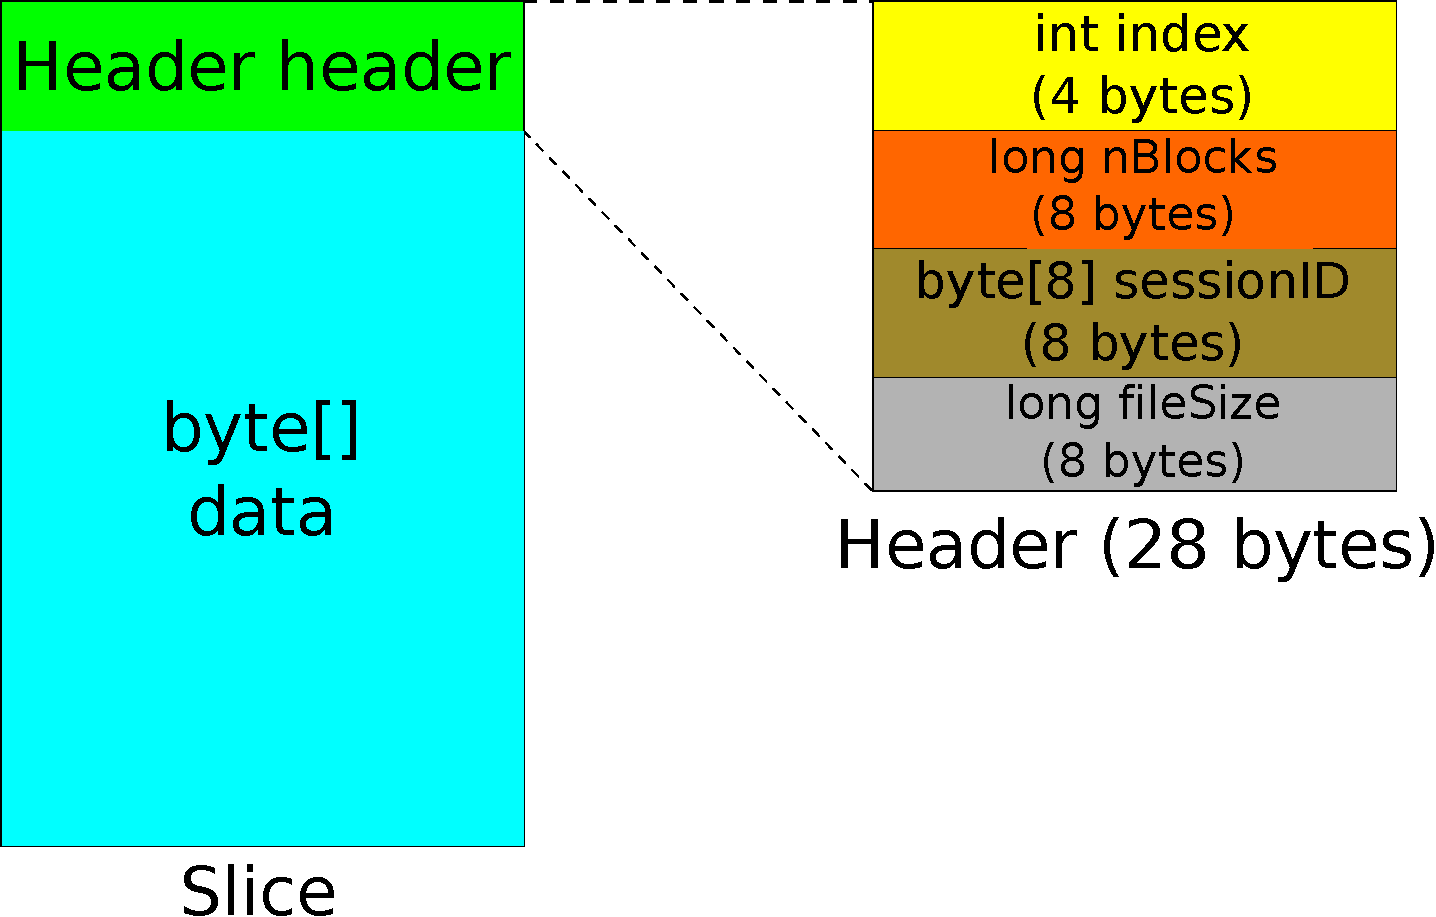
\includegraphics[scale=0.4]{Figures/Slice_Header_1}
  \decoRule
  \caption[\code{Slice} - \code{Header} (Versión 1)]{Esquema general de las clases \code{Slice} y \code{Header} (Versión 1)}
  \label{fig:Slice_Header_1}
\end{figure}

\begin{itemize}
  \item \keyword{\code{Slice}} -- Un objeto de clase \code{Slice} es uno de los fragmentos en los que un fichero original se ha dividido. Está formado por una cabecera (\code{Header}) y un array de \emph{bytes} en el que se almacena el contenido del segmento del fichero. (Figura~\ref{fig:Slice_Header_1}) \footnote{Debido al contexto del TFG, se ha decidido no usar UML para confeccionar los esquemas expuestos en este capítulo.}

  \item \keyword{\code{Header}} -- En esta clase se almacenan los metadatos de un objeto de clase \code{Slice}. Se guardan datos como un contador, el número total de fragmentos para un fichero, un ID para la sesión\footnote{En esta primera iteración de la aplicación, el ID para identificar la sesión es un resumen \emph{hash} del fichero.} y el tamaño original del fichero. (Figura~\ref{fig:Slice_Header_1})
\end{itemize}

También se han desarrollado otras clases con métodos para trocear y recomponer un fichero:

\begin{figure}[!htb]
  \centering
  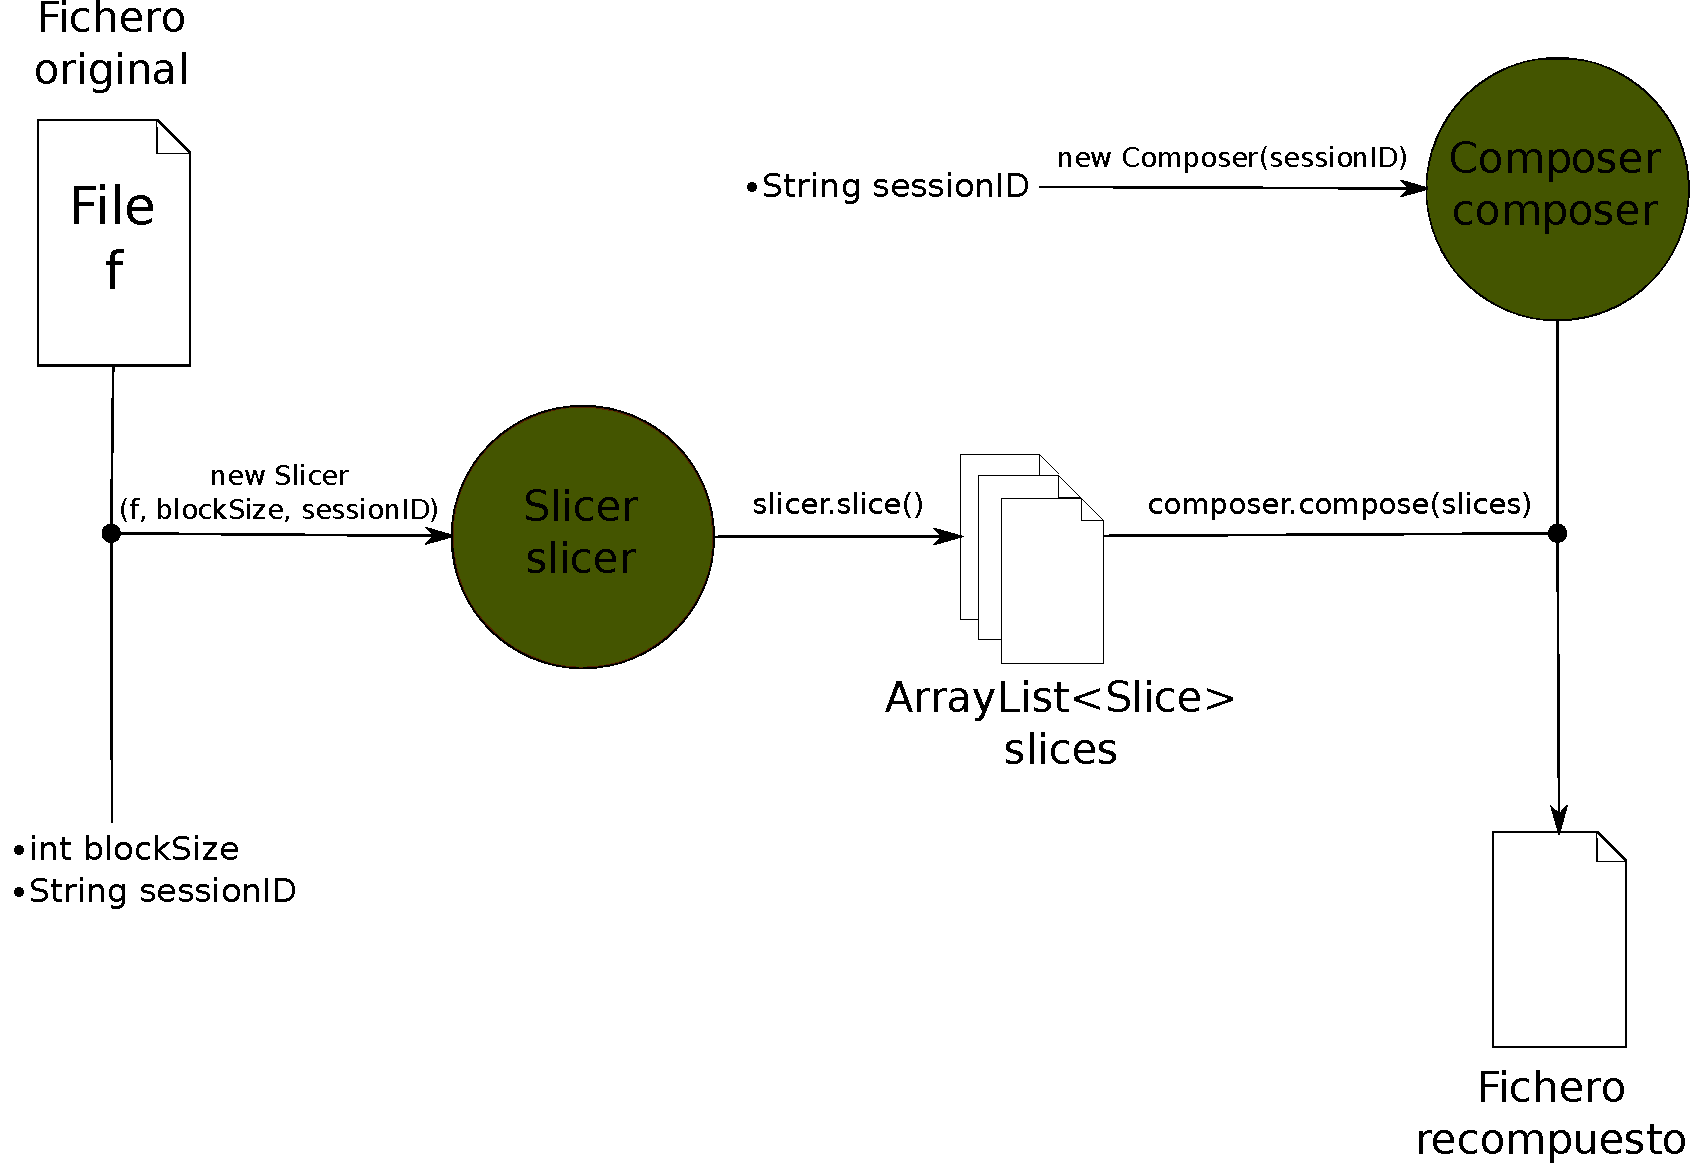
\includegraphics[scale=0.5]{Figures/Assembler}
  \decoRule
  \caption[\code{Slicer} - \code{Composer}]{Esquema general del funcionamiento de las clases \code{Slicer} y \code{Composer}}
  \label{fig:Assembler}
\end{figure}

\begin{itemize}
  \item \keyword{\code{Slicer}} -- Esta clase posee métodos para crear objetos de clase \code{Slice}. Recibe un fichero, un tamaño de bloque y un ID para identificar la sesión. Lee del fichero bloques del tamaño indicado hasta alcanzar el EOF y genera un \code{Slice} para cada uno de ellos, con una cabecera distinta. (Figura~\ref{fig:Assembler})

  \item \keyword{\code{Composer}} -- Esta clase, a través de un método, recibe un array de objetos de clase \code{Slice} y devuelve un fichero compuesto. Lee uno a uno los fragmentos que recibe, prestando especial atención a sus cabeceras y si detecta que alguno falta genera un log de errores. (Figura~\ref{fig:Assembler})
\end{itemize}

\subsection{Shatter II}

En esta segunda versión, el objetivo del prototipo es proporcionar confidencialidad a los objetos de clase \code{Slice}. Para llevarlo a cabo se han implementado las siguientes clases:

\begin{figure}[!htb]
  \centering
  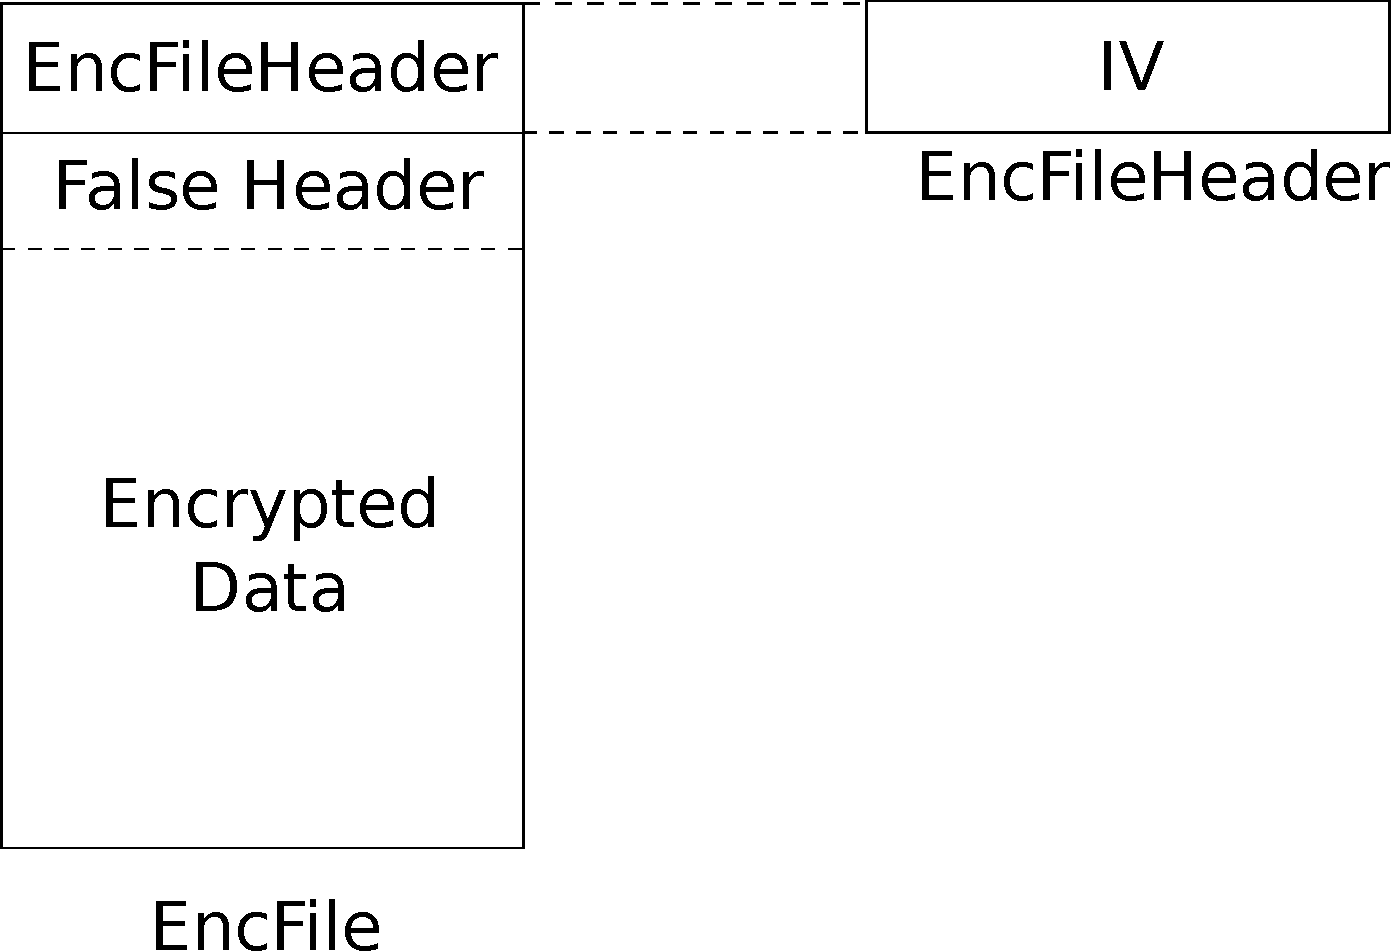
\includegraphics[scale=0.4]{Figures/EncFile_Header_1}
  \decoRule
  \caption[\code{EncFile} - \code{EncFileHeader} (Versión 1)]{Esquema general de las clases \code{EncFile} y \code{EncFileHeader} (Versión 1)}
  \label{fig:EncFile_Header_1}
\end{figure}

\begin{itemize}
  \item \keyword{\code{EncFile}} -- Viene a ser un objeto de clase \code{Slice} cifrado. A parte de los datos encriptados del \code{Slice}, también incluye una cabecera (\code{EncFileHeader}) con algunos datos importantes y una pseudocabecera (\code{FalseHeader}) con datos menores. (Figura~\ref{fig:EncFile_Header_1})

  \item \keyword{\code{EncFileHeader}} -- Esta cabecera se usa para almacenar algunos metadatos importantes como, en este caso, el vector de inicialización (IV) que se ha usado en el cifrado del objeto \code{Slice}. (Figura~\ref{fig:EncFile_Header_1})

  \item \keyword{\code{KeyFile}} -- Esta clase se utiliza para almacenar la clave simétrica que se ha utilizado para crear los objetos de clase \code{EncFile}.
\end{itemize}

Además de estas clases, se han creado otras clases que aportan los métodos necesarios para cifrar los fragmentos:

\begin{figure}[!htb]
  \centering
  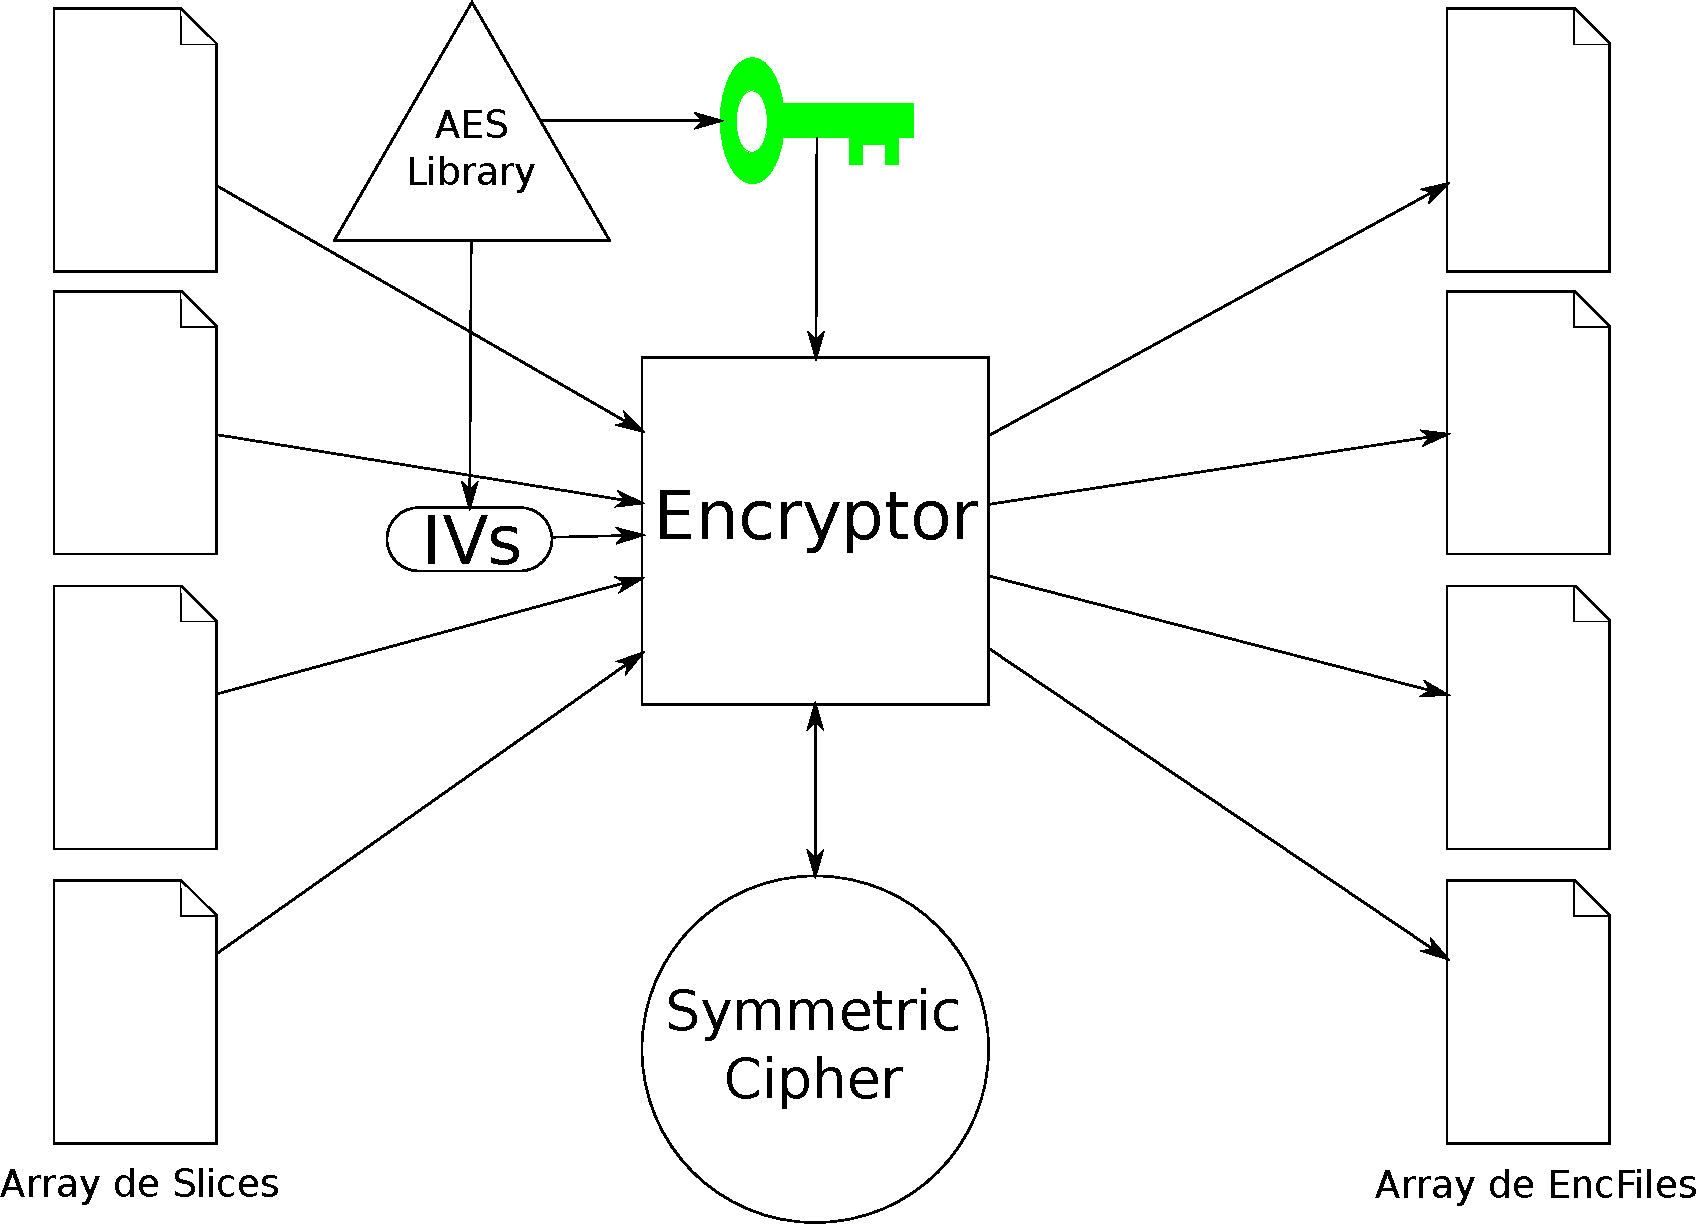
\includegraphics[scale=0.5]{Figures/Encryptor}
  \decoRule
  \caption[\code{Encryptor}]{Esquema general del funcionamiento de la clase \code{Encryptor}}
  \label{fig:Encryptor}
\end{figure}

\begin{figure}[!htb]
  \centering
  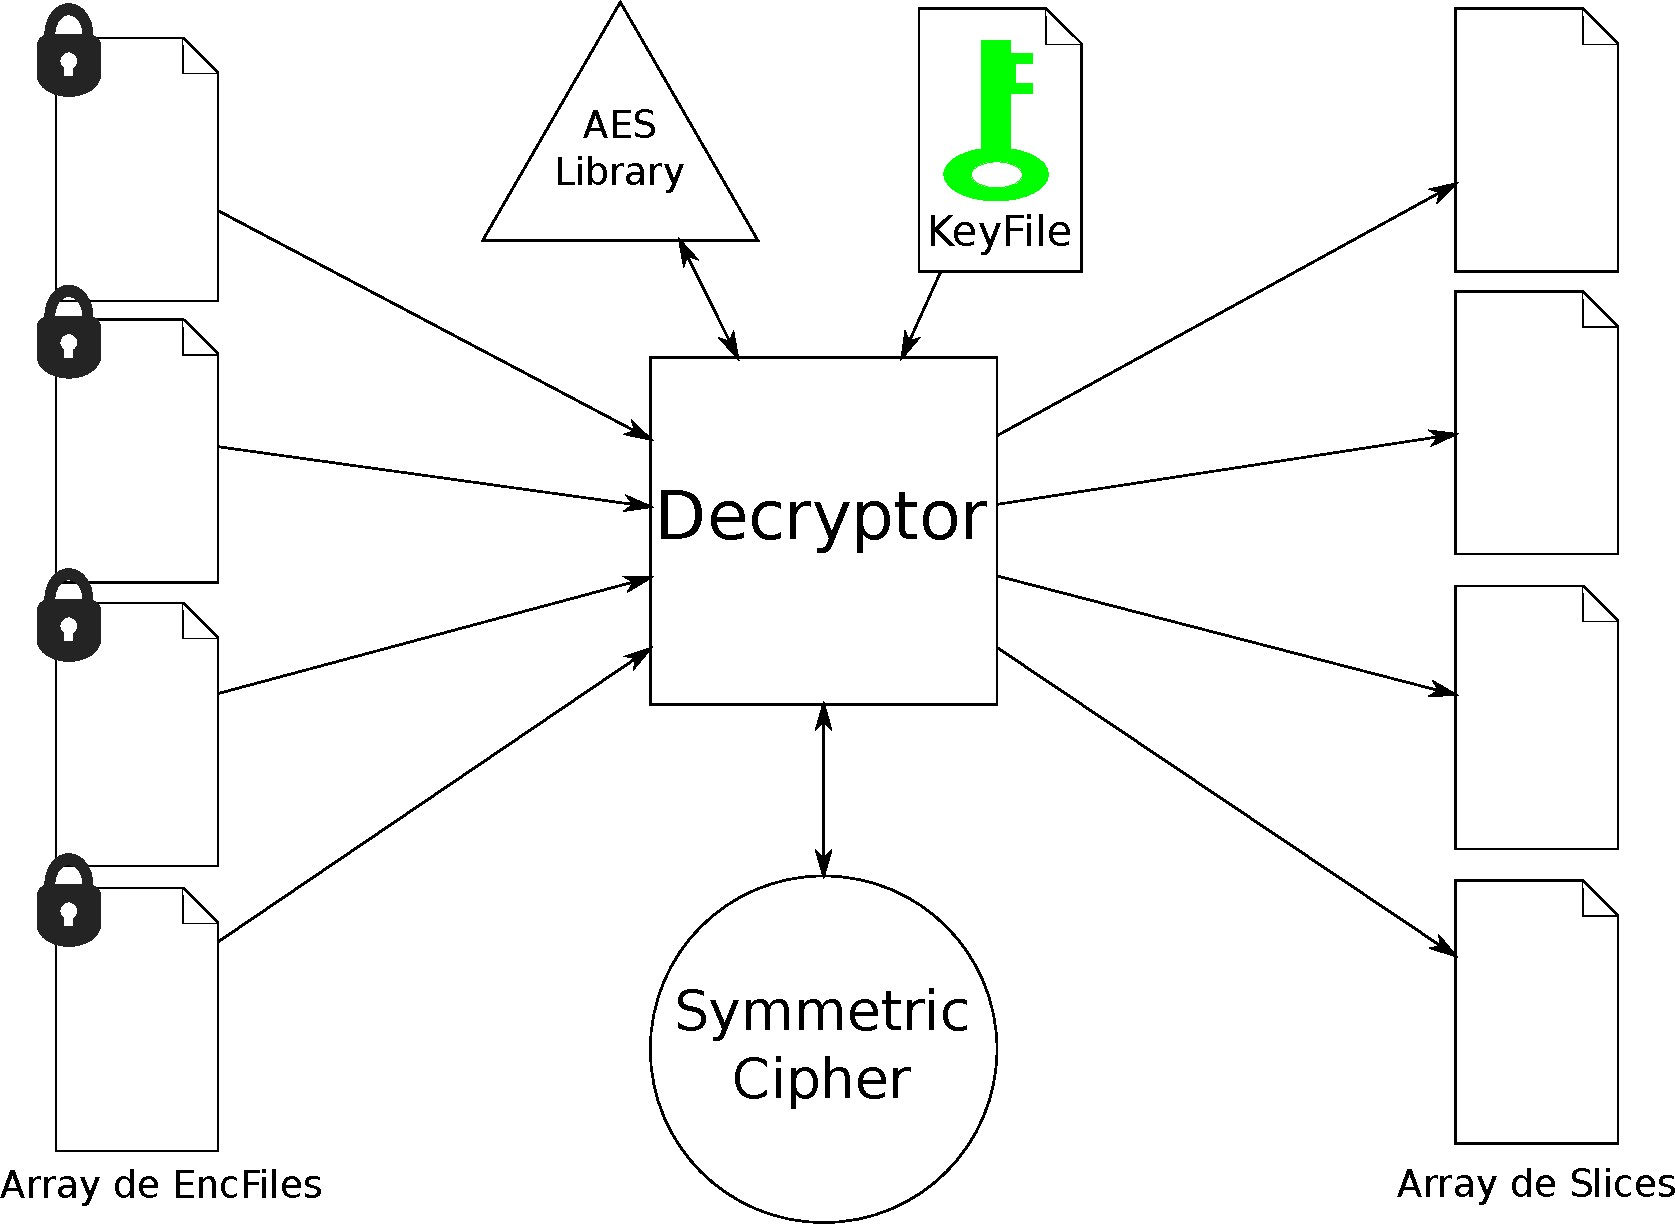
\includegraphics[scale=0.5]{Figures/Decryptor}
  \decoRule
  \caption[\code{Decryptor}]{Esquema general del funcionamiento de la clase \code{Decryptor}}
  \label{fig:Decryptor}
\end{figure}

\begin{itemize}
  \item \keyword{\code{AESLibrary}} -- Básicamente, una clase que se encarga de generar de manera aleatoria y segura claves simétricas y vectores de inicialización.

  \item \keyword{\code{SymmetricCipher}} -- Esta es la clase que se encarga de hacer la parte más importante en cuanto a la confidencialidad. Una vez que ha sido inicializada con una clave simétrica, genera textos cifrados a partir de texto plano y un IV. Igualmente, puede llevar a cabo el proceso inverso.

  \item \keyword{\code{Encryptor}} -- Esta clase, en conjunto con las dos anteriores, es la encargada de generar los objetos de clase \code{EncFile}. Genera de manera aleatoria y segura una clave simétrica para un algoritmo establecido y, con ella, inicializa una instancia de la clase \code{SymmetricCipher}. A continuación se le pasa un array de objetos de clase \code{Slice} del cual genera un array de objetos de clase \code{EncFile}, que es el que devuelve a través de un método. (Figura~\ref{fig:Encryptor})

  \item \keyword{\code{Decryptor}} -- La contraparte de la clase \code{Encryptor}. Realiza el proceso inverso y devuelve un array de objetos de clase \code{Slice} a partir de uno de objetos de clase \code{EncFile}. (Figura~\ref{fig:Decryptor})
\end{itemize}

\subsection{Shatter III}

El objetivo en esta tercera iteración es el de proporcionar integridad y autenticación a las clases ya implementadas, al igual que confidencialidad a la clave simétrica que se utiliza para generarlas. Para lograrlo, se han implementado algunas clases nuevas:

\begin{itemize}
  \item \keyword{\code{EncKeyFile}} -- Esta clase almacena la clave simétrica protegida mediante cifrado asimétrico usando la clave pública del destinatario del mensaje, con lo que se logra la confidencialidad de la clave entre los usuarios. Tiene una cabecera (\code{EncKeyFileHeader}) en la que se guardan algunos datos importantes.

  \item \keyword{\code{EncKeyFileHeader}} -- La cabecera de un objeto de clase \code{EncKeyFile}. En ella se almacena una HMAC cifrada de la clave simétrica.

  \item \keyword{\code{Signature}} -- Básicamente una clase para contener una HMAC.

  \item \keyword{\code{SecureSignature}} -- Contiene la HMAC comentada antes pero cifrada usando una clave asimétrica. De esta forma también le damos confidencialidad a la firma.
\end{itemize}

Para poder llevar a cabo el cifrado asimétrico se han desarrollado otras clases:

\begin{figure}[!htb]
  \centering
  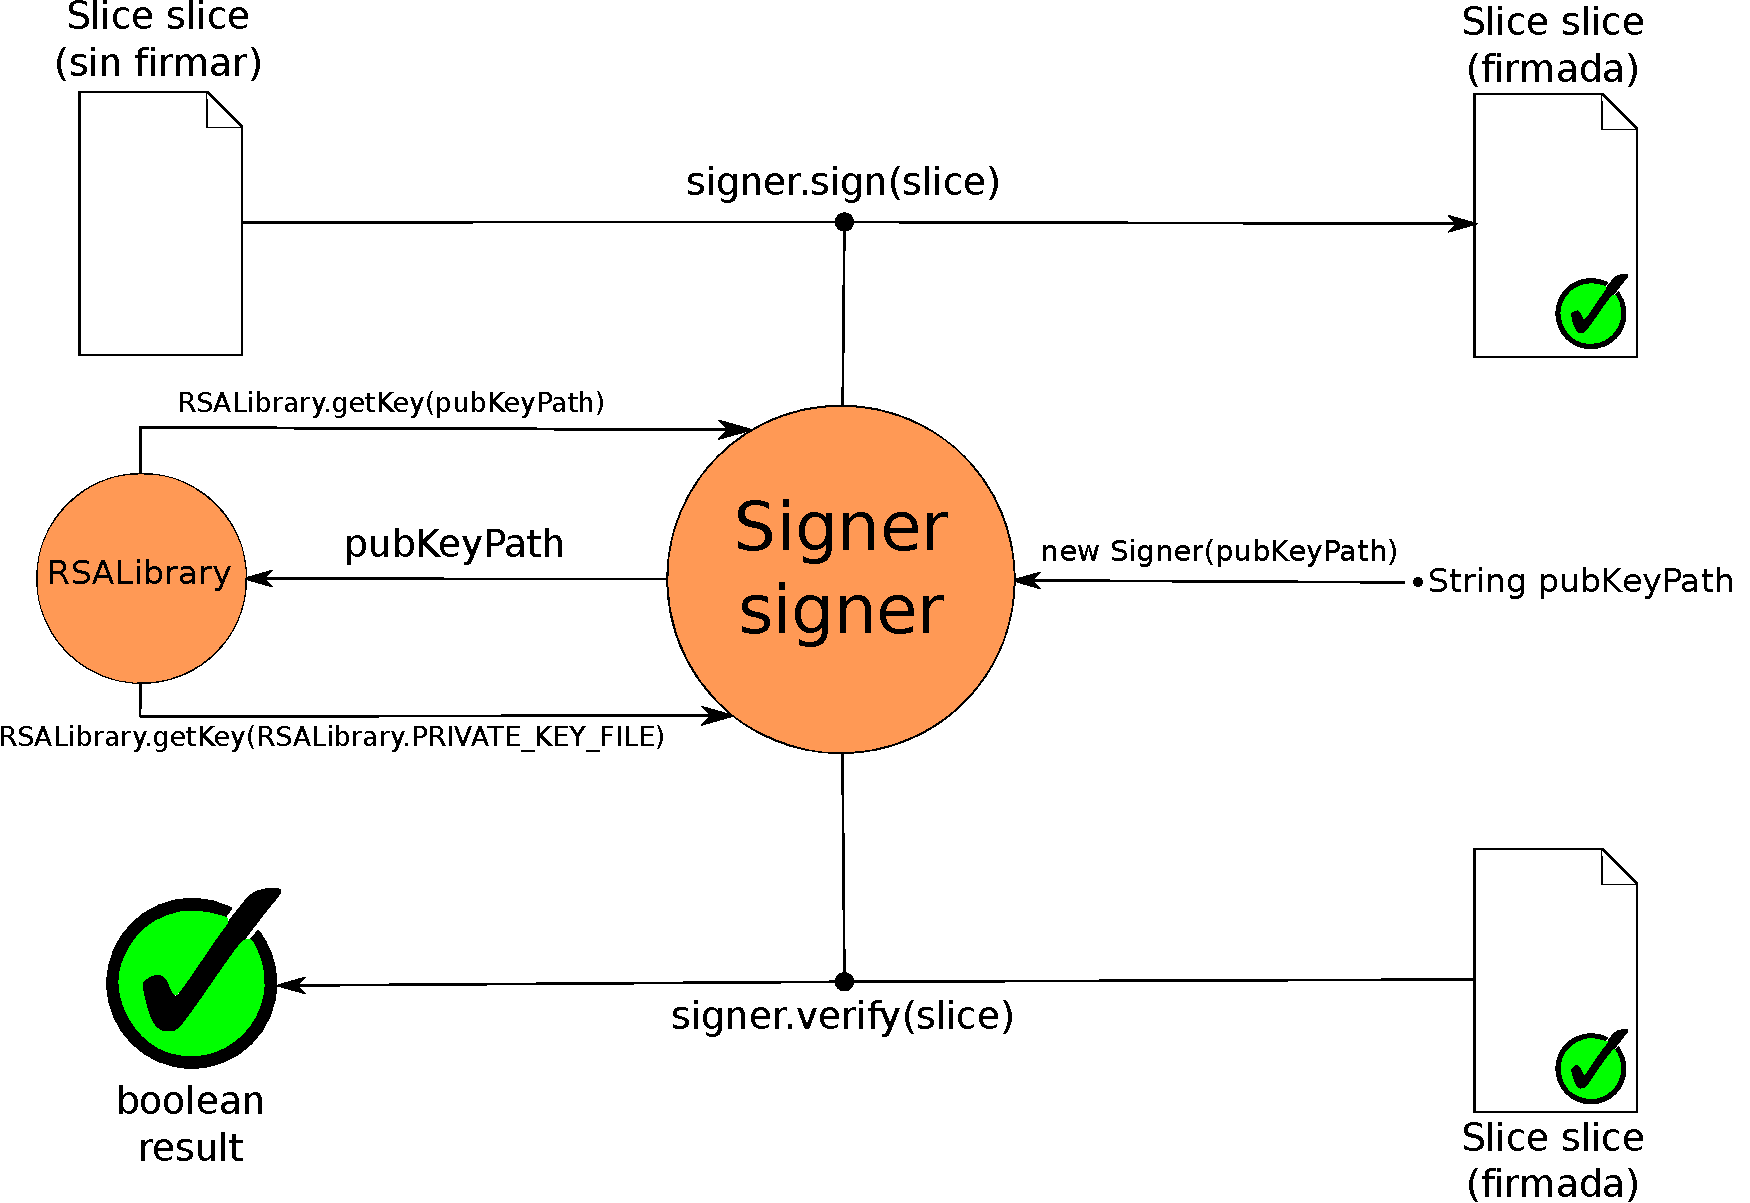
\includegraphics[scale=0.5]{Figures/Signer_1}
  \decoRule
  \caption[\code{Signer} (Versión 1)]{Esquema general del funcionamiento de la clase \code{Signer} (Versión 1)}
  \label{fig:Signer_1}
\end{figure}

\begin{itemize}
  \item \keyword{\code{RSALibrary}} -- Esta clase es la encargada de generar un par de claves asimétricas, de escribirlas y leerlas de un fichero, de cifrar un texto plano y de descifrar uno cifrado.

  \item \keyword{\code{Signer}} -- La clase que se encarga de recibir objetos de clase \code{Slice}, \code{EncFile}, \code{KeyFile} y demás y devolverlos firmados. Asimismo, se encarga de comprobar las firmas de todas estas clases para preservar la autenticidad de la información que portan. (Figura~\ref{fig:Signer_1})

  \item \keyword{\code{RSAPSS}} -- Esta clase incorpora todos los métodos necesarios para generar, a partir de un texto plano, un texto codificado y firmado usando el algoritmo RSASSA-PSS. También realiza el proceso inverso y puede verificar las firmas.
\end{itemize}

En este prototipo se ha añadido una firma a varias de las clases que ya estaban implementadas:

\begin{figure}[!htb]
  \centering
  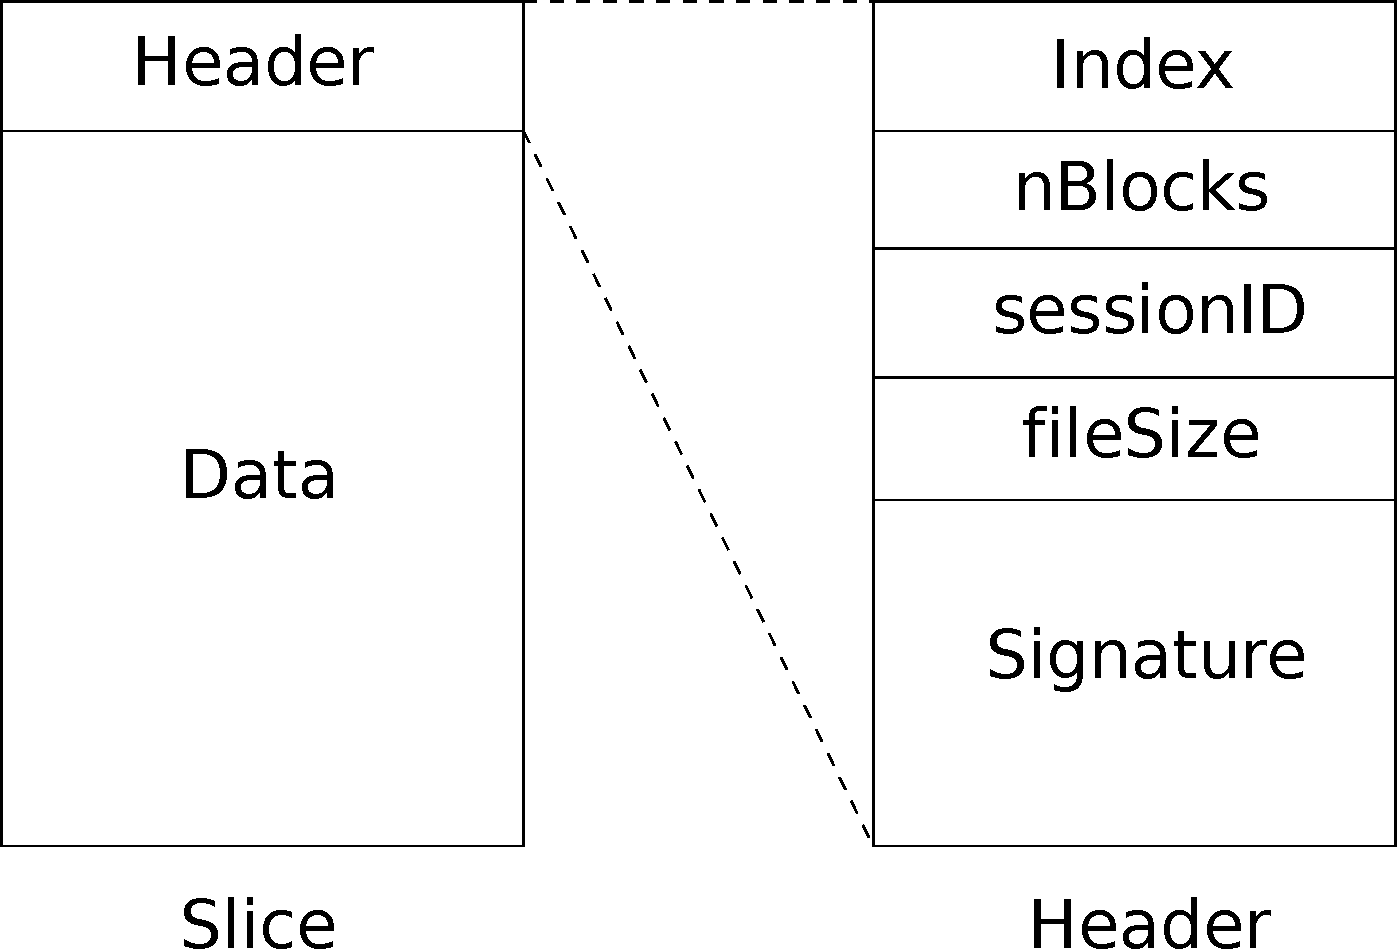
\includegraphics[scale=0.4]{Figures/Slice_Header_2}
  \decoRule
  \caption[\code{Slice} - \code{Header} (Versión final)]{Esquema general de las clases \code{Slice} y \code{Header} (Versión final)}
  \label{fig:Slice_Header_2}
\end{figure}

\begin{figure}[!htb]
  \centering
  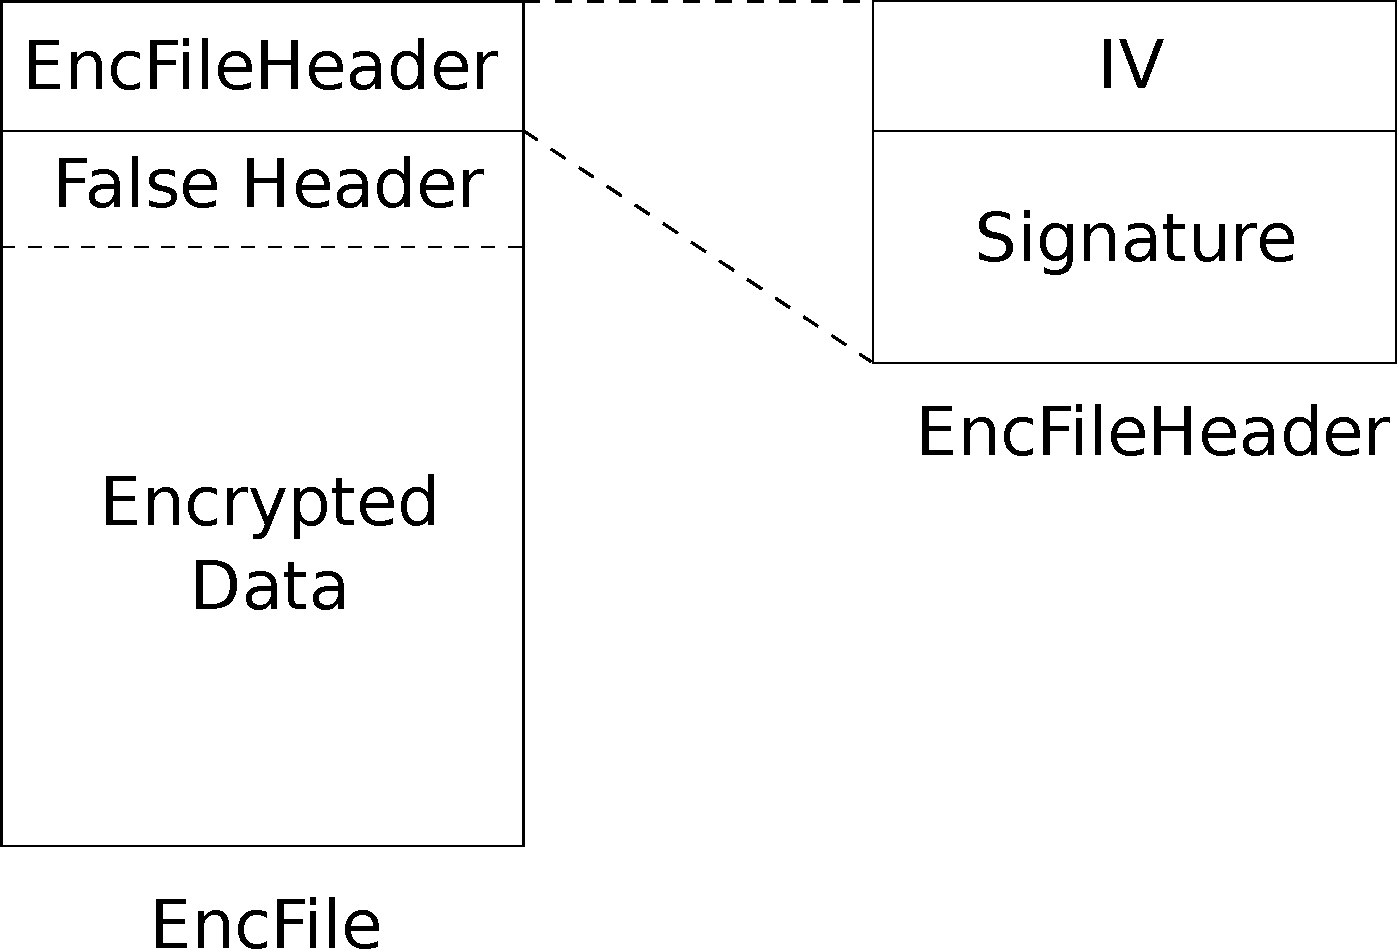
\includegraphics[scale=0.4]{Figures/EncFile_Header_2}
  \decoRule
  \caption[\code{EncFile} - \code{EncFileHeader} (Versión final)]{Esquema general de las clases \code{EncFile} y \code{EncFileHeader} (Versión final)}
  \label{fig:EncFile_Header_2}
\end{figure}

\begin{itemize}
  \item A la clase \code{Slice} se le ha añadido en la cabecera una firma, que otorga integridad y autenticación a los datos que lleva. (Figura~\ref{fig:Slice_Header_2})

  \item A la clase \code{EncFile} se le ha añadido también una firma, esta vez para darle la integridad y la autenticación al IV que se encuentra en su cabecera. (Figura~\ref{fig:EncFile_Header_2})

  \item La clase \code{KeyFile} tiene una firma de la clave simétrica.
\end{itemize}

Además de las clases mencionadas anteriormente, también se han desarrollado otras clases funcionales:

\begin{itemize}
  \item \keyword{\code{RandomString}} -- Esta clase posee un método que devuelve un \code{String} aleatorio de 8 caracteres.

  \item \keyword{\code{FileIO}} -- Esta clase tiene métodos para escribir y leer los distintos ficheros que intervienen en la aplicación.

  \item \keyword{\code{Bytes}} -- Tiene implementados varios métodos para hacer operaciones con arrays de \emph{bytes}.
\end{itemize}

\subsection{Shatter IV}

Este último prototipo está desarrollado como una aplicación en Android. El objetivo de este prototipo es hacer uso de varias herramientas que posee Android para que la aplicación funcione correctamente. Para ello se han creado nuevas clases:

\begin{itemize}
  \item \keyword{\code{KeyStoreHandler}} -- Esta clase se usa para realizar todas las operaciones necesarias con el \emph{Keystore} de Android (Véase~\ref{Keystore}). Se encarga de almacenar las claves, recuperarlas, usarlas para encriptar, firmar, etc.

  \item \keyword{\code{HTTPClient}} -- Un cliente HTTP muy sencillo que únicamente realiza peticiones GET.

  \item \keyword{\code{ExternalStorage}} -- Esta clase se encarga de interactuar con el \emph{External Storage} de Android. Incorpora algunos métodos para conseguir \emph{paths}, descriptores de fichero o crear directorios.
\end{itemize}

Para que los usuarios puedan enviar sus mensajes, se ha dispuesto un servidor HTTP bastante sencillo al que los usuarios pueden subir sus mensajes. Gracias a la clase \code{HTTPClient}, el destinatario puede bajarse los fragmentos de un mensaje.

\begin{figure}[!htb]
  \centering
  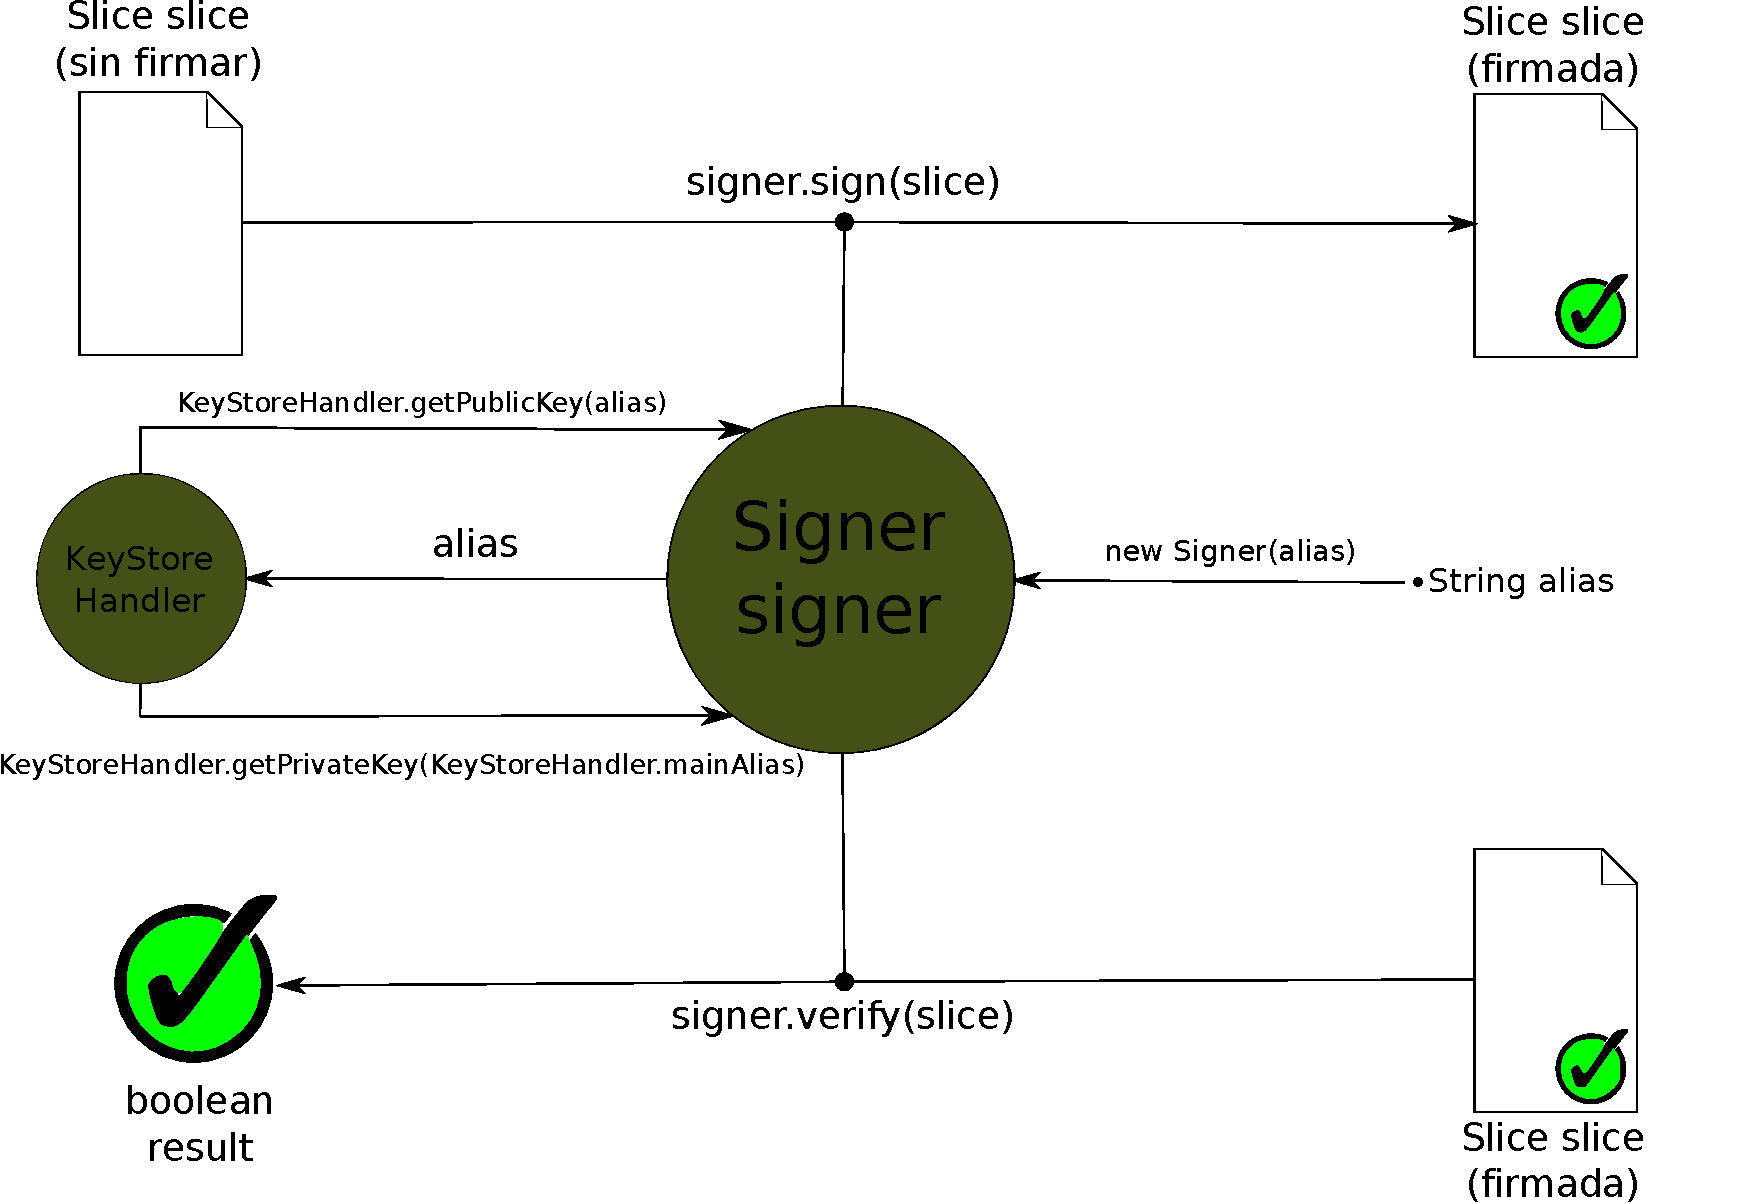
\includegraphics[scale=0.5]{Figures/Signer_2}
  \decoRule
  \caption[\code{Signer} (Versión final)]{Esquema general del funcionamiento de la clase \code{Signer} (Versión final)}
  \label{fig:Signer_2}
\end{figure}

El uso del \emph{Keystore} de Android obliga a utilizar las claves que se almacenan en él usando unos métodos específicos. Debido a ello, algunas clases ya creadas (Como \code{RSALibrary} o \code{RSAPSS}) se sustituyen por métodos específicos que se implementan en la clase \code{KeyStoreHandler}. (Figura~\ref{fig:Signer_2})

El ID que aparece en las cabeceras de la clase \code{Slice} se sustituye por un \code{String} aleatorio que genera la clase \code{RandomString}. Este cambio se debe a que el resumen \emph{hash} que se usaba anteriormente queda en desuso al añadir la firma a estas clases. Además, este ID aleatorio identifica a todos los objetos de clase \code{Slice} que pertenecen a un mismo mensaje.

El esquema general de la aplicación se puede dividir en dos: Una primera parte se encarga de la división y cifrado del fichero (Figura~\ref{fig:abstractA}). La otra se encarga de descargar del servidor los fragmentos cifrados y recomponer el fichero original (Figura~\ref{fig:abstractB}).

\begin{figure}[!htb]
  \centering
  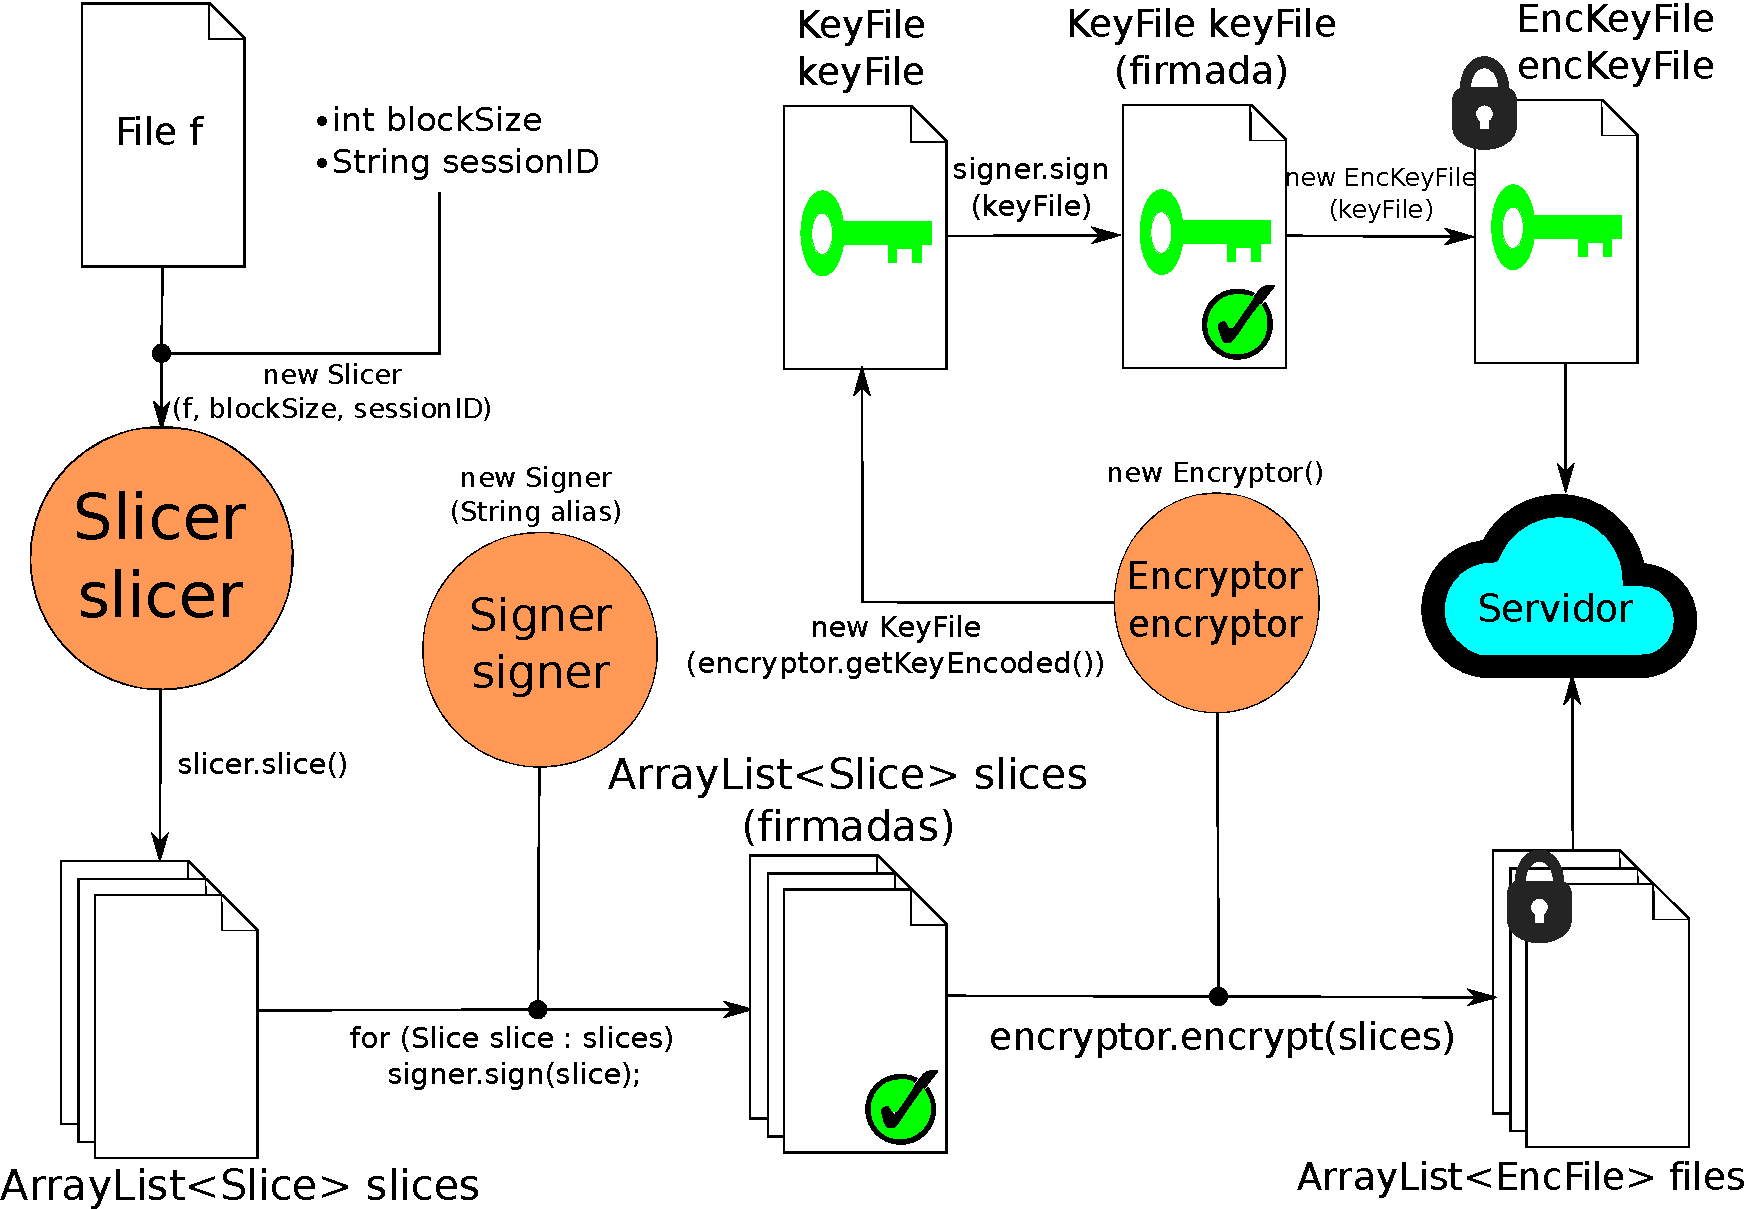
\includegraphics[scale=0.5]{Figures/abstractA}
  \decoRule
  \caption[\code{SliceEncrypt}]{Esquema general de la clase \code{SliceEncrypt}, la primera parte en el proceso de comunicación de la aplicación}
  \label{fig:abstractA}
\end{figure}

\begin{figure}[!htb]
  \centering
  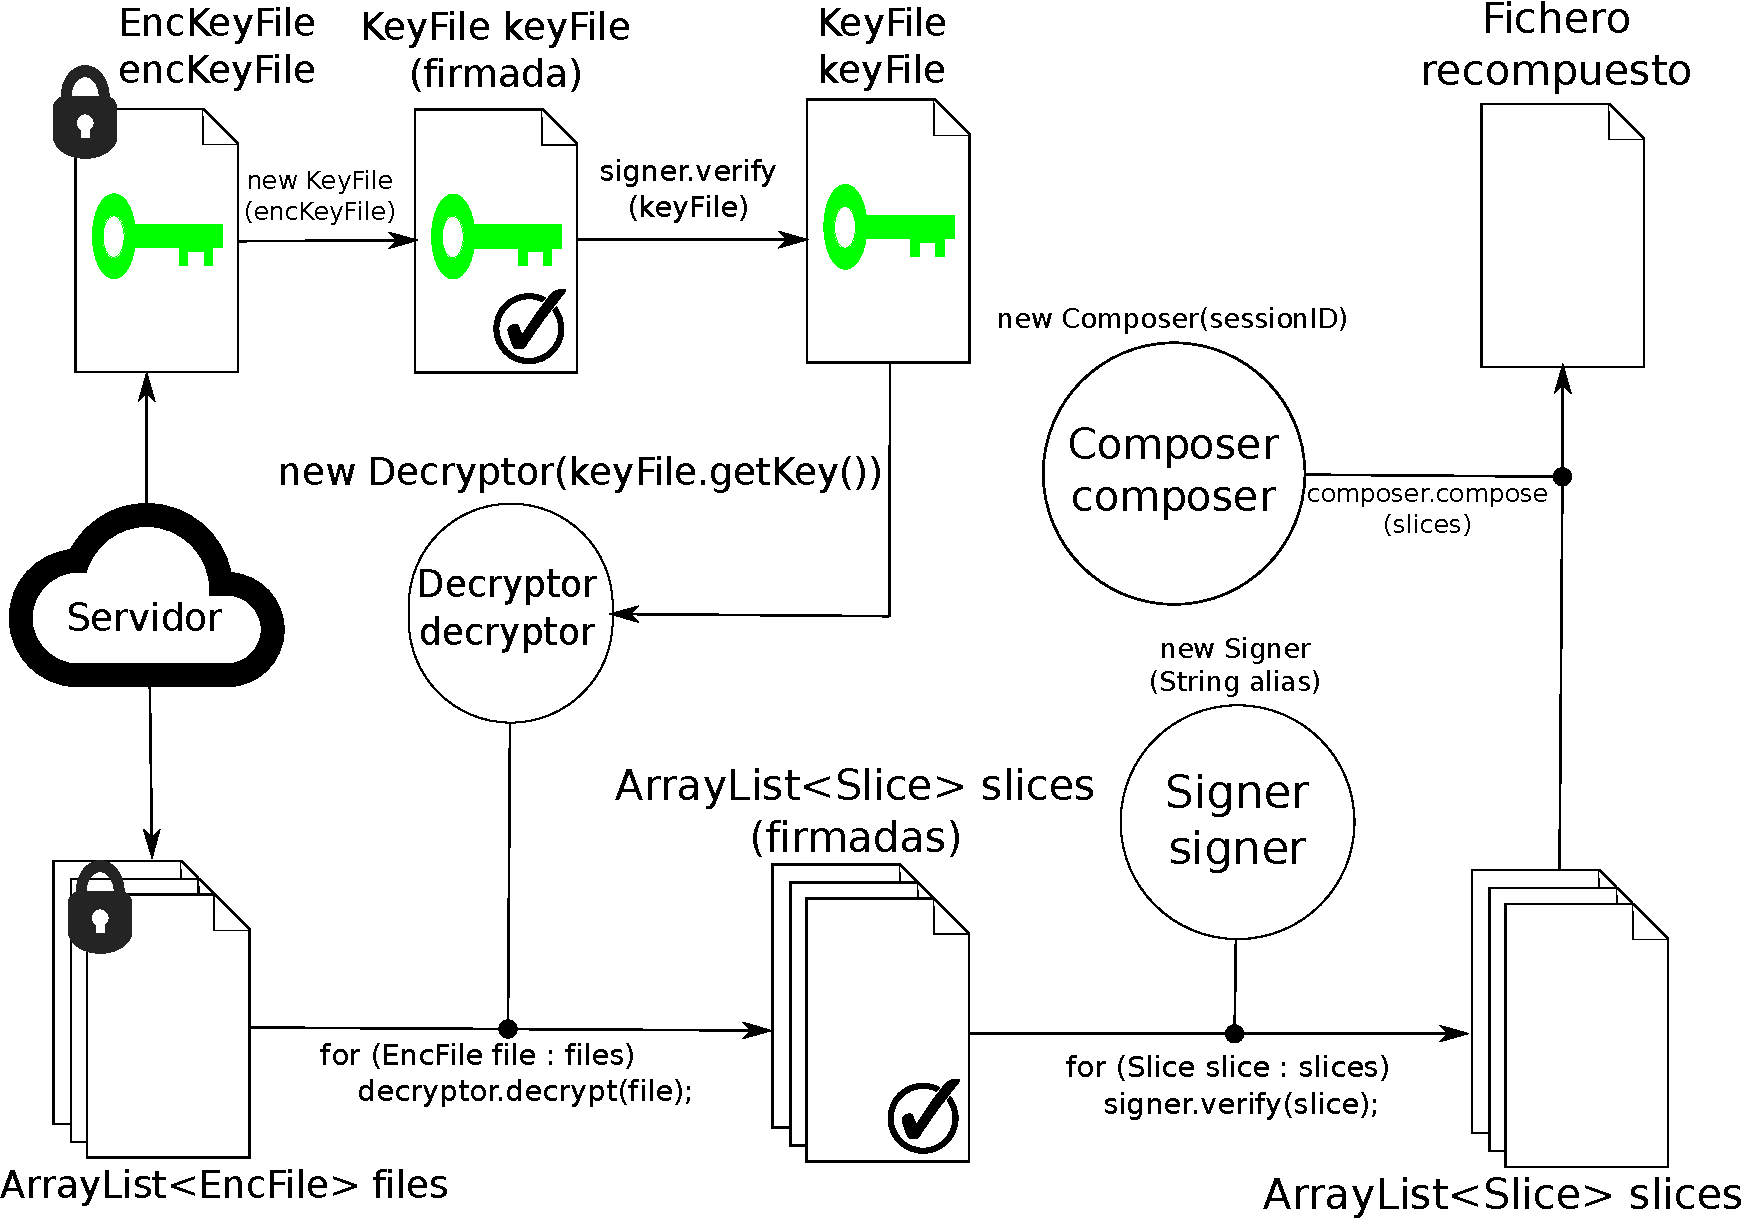
\includegraphics[scale=0.5]{Figures/abstractB}
  \decoRule
  \caption[\code{DecryptCompose}]{Esquema general de \code{DecryptCompose}, la parte final en el proceso de comunicación de la aplicación}
  \label{fig:abstractB}
\end{figure}

%-------------------------------------------------------------------------------

\section{Tiempo dedicado}

El desarrollo de cada prototipo ha necesitado un tiempo de trabajo distinto. En esta sección se detalla el número de horas dedicado a cada uno de ellos:

\begin{itemize}
  \item El primer prototipo, al tratarse de un esquema bastante sencillo, no ha supuesto un número de horas excesivo. El desarrollo de este prototipo se finalizó a las dos semanas de iniciar el proyecto, habiendo dedicado una media de dos horas diarias (28 horas).

  \item El segundo prototipo ha supuesto no solo tiempo de desarrollo, también ha necesitado tiempo de investigación para elegir el algoritmo más adecuado para el proyecto. Para este prototipo se dedicó, a partir de la finalización del prototipo anterior, dos semanas de desarrollo y una de investigación, dedicando una media de dos horas diarias (42 horas).

  \item El tercer prototipo ha necesitado una primera parte de investigación para elegir el algoritmo de cifrado asimétrico y firma adecuados y luego una parte de desarrollo. El desarrollo de este prototipo ha requerido, a partir de la finalización del prototipo anterior, dos semanas de investigación y cuatro de desarrollo, dedicando una media de dos horas diarias (84 horas).

  \item El cuarto prototipo, al tratarse de una migración a otra plataforma, no debería haber supuesto mucho tiempo de trabajo. Sin embargo se ha dedicado más tiempo debido a los problemas que se detallan en el Capítulo~\ref{Chapter5.2}. Esta fase ha requerido una primera semana de investigación para encontrar la mejor forma de realizar la migración, y cinco semanas de desarrollo para llevarlo a cabo, dedicando una media de dos horas diarias (84 horas).
\end{itemize}

En total, el desarrollo del proyecto ha conllevado aproximadamente 238 horas de trabajo, habiendo invertido más tiempo en el desarrollo que en la investigación.

% Chapter 5: Results

\chapter{Resultados} % Main chapter title

\label{Chapter5} % Reference

%-------------------------------------------------------------------------------

\section{Ejemplos de uso de la aplicación}

%En esta sección se va a poner un ejemplo de como un usuario utilizaría la aplicación ya descargada en su terminal móvil.
Esta sección muestra un ejemplo de uso completo de la aplicación, pasando por los prerrequisitos, el cifrado de un fichero y la descarga de un mensaje.

\begin{figure}[!htb]
  \centering
  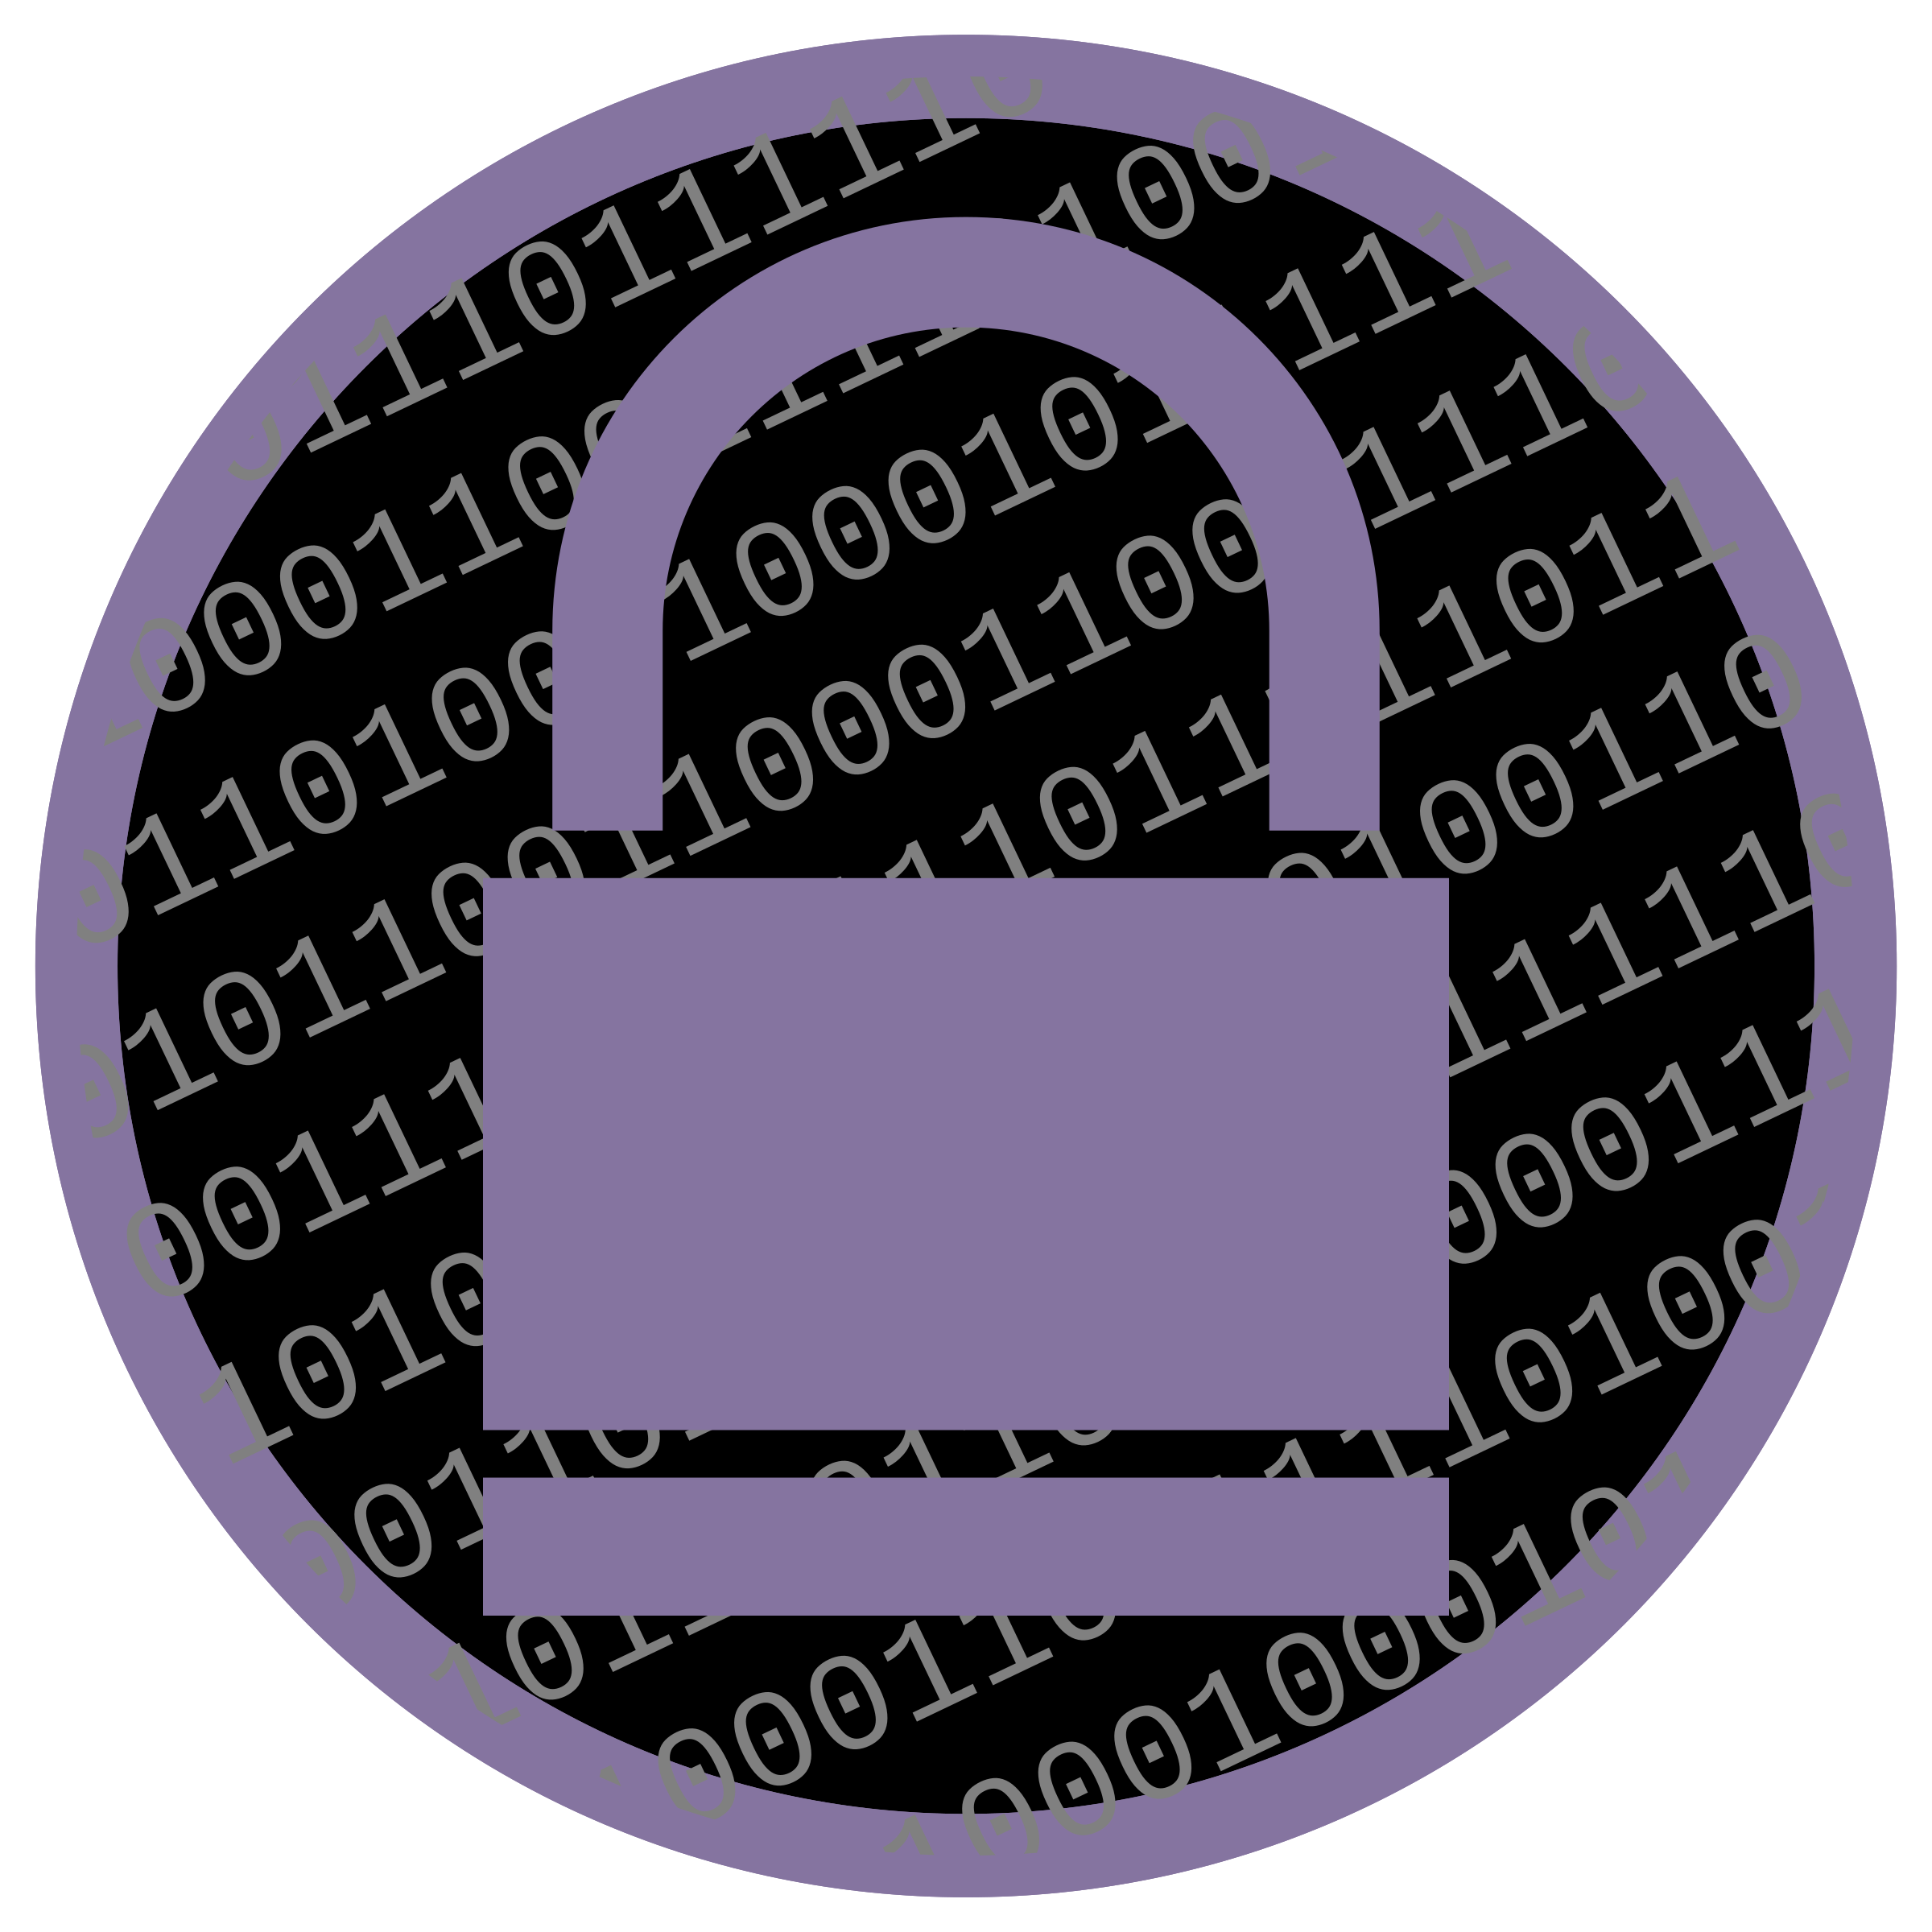
\includegraphics[scale=0.2]{Figures/launcher}
  \decoRule
  \caption[Shatter (Icono)]{Icono de la aplicación Shatter}
  \label{fig:launcher}
\end{figure}

\subsection{Prerrequisitos}

Al tratarse de una aplicación Android, es necesario el uso de un dispositivo que utilice el sistema operativo Android (Véase~\ref{Android}), específicamente la versión 6 (Marshmallow) o una superior.

También es necesario dar permisos de escritura en el almacenamiento del dispositivo, ya que la aplicación realiza operaciones de escritura y lectura.

\subsection{Añadir contactos}

Al abrir la aplicación por primera vez se genera un par de claves asimétricas, una pública y otra privada. En la pantalla principal, al no disponer de ningún contacto, solo se puede ver un campo de texto, un botón para seleccionar un fichero y un botón para añadir usuarios. (Figura~\ref{fig:home})

\begin{figure}[!htb]
  \centering
  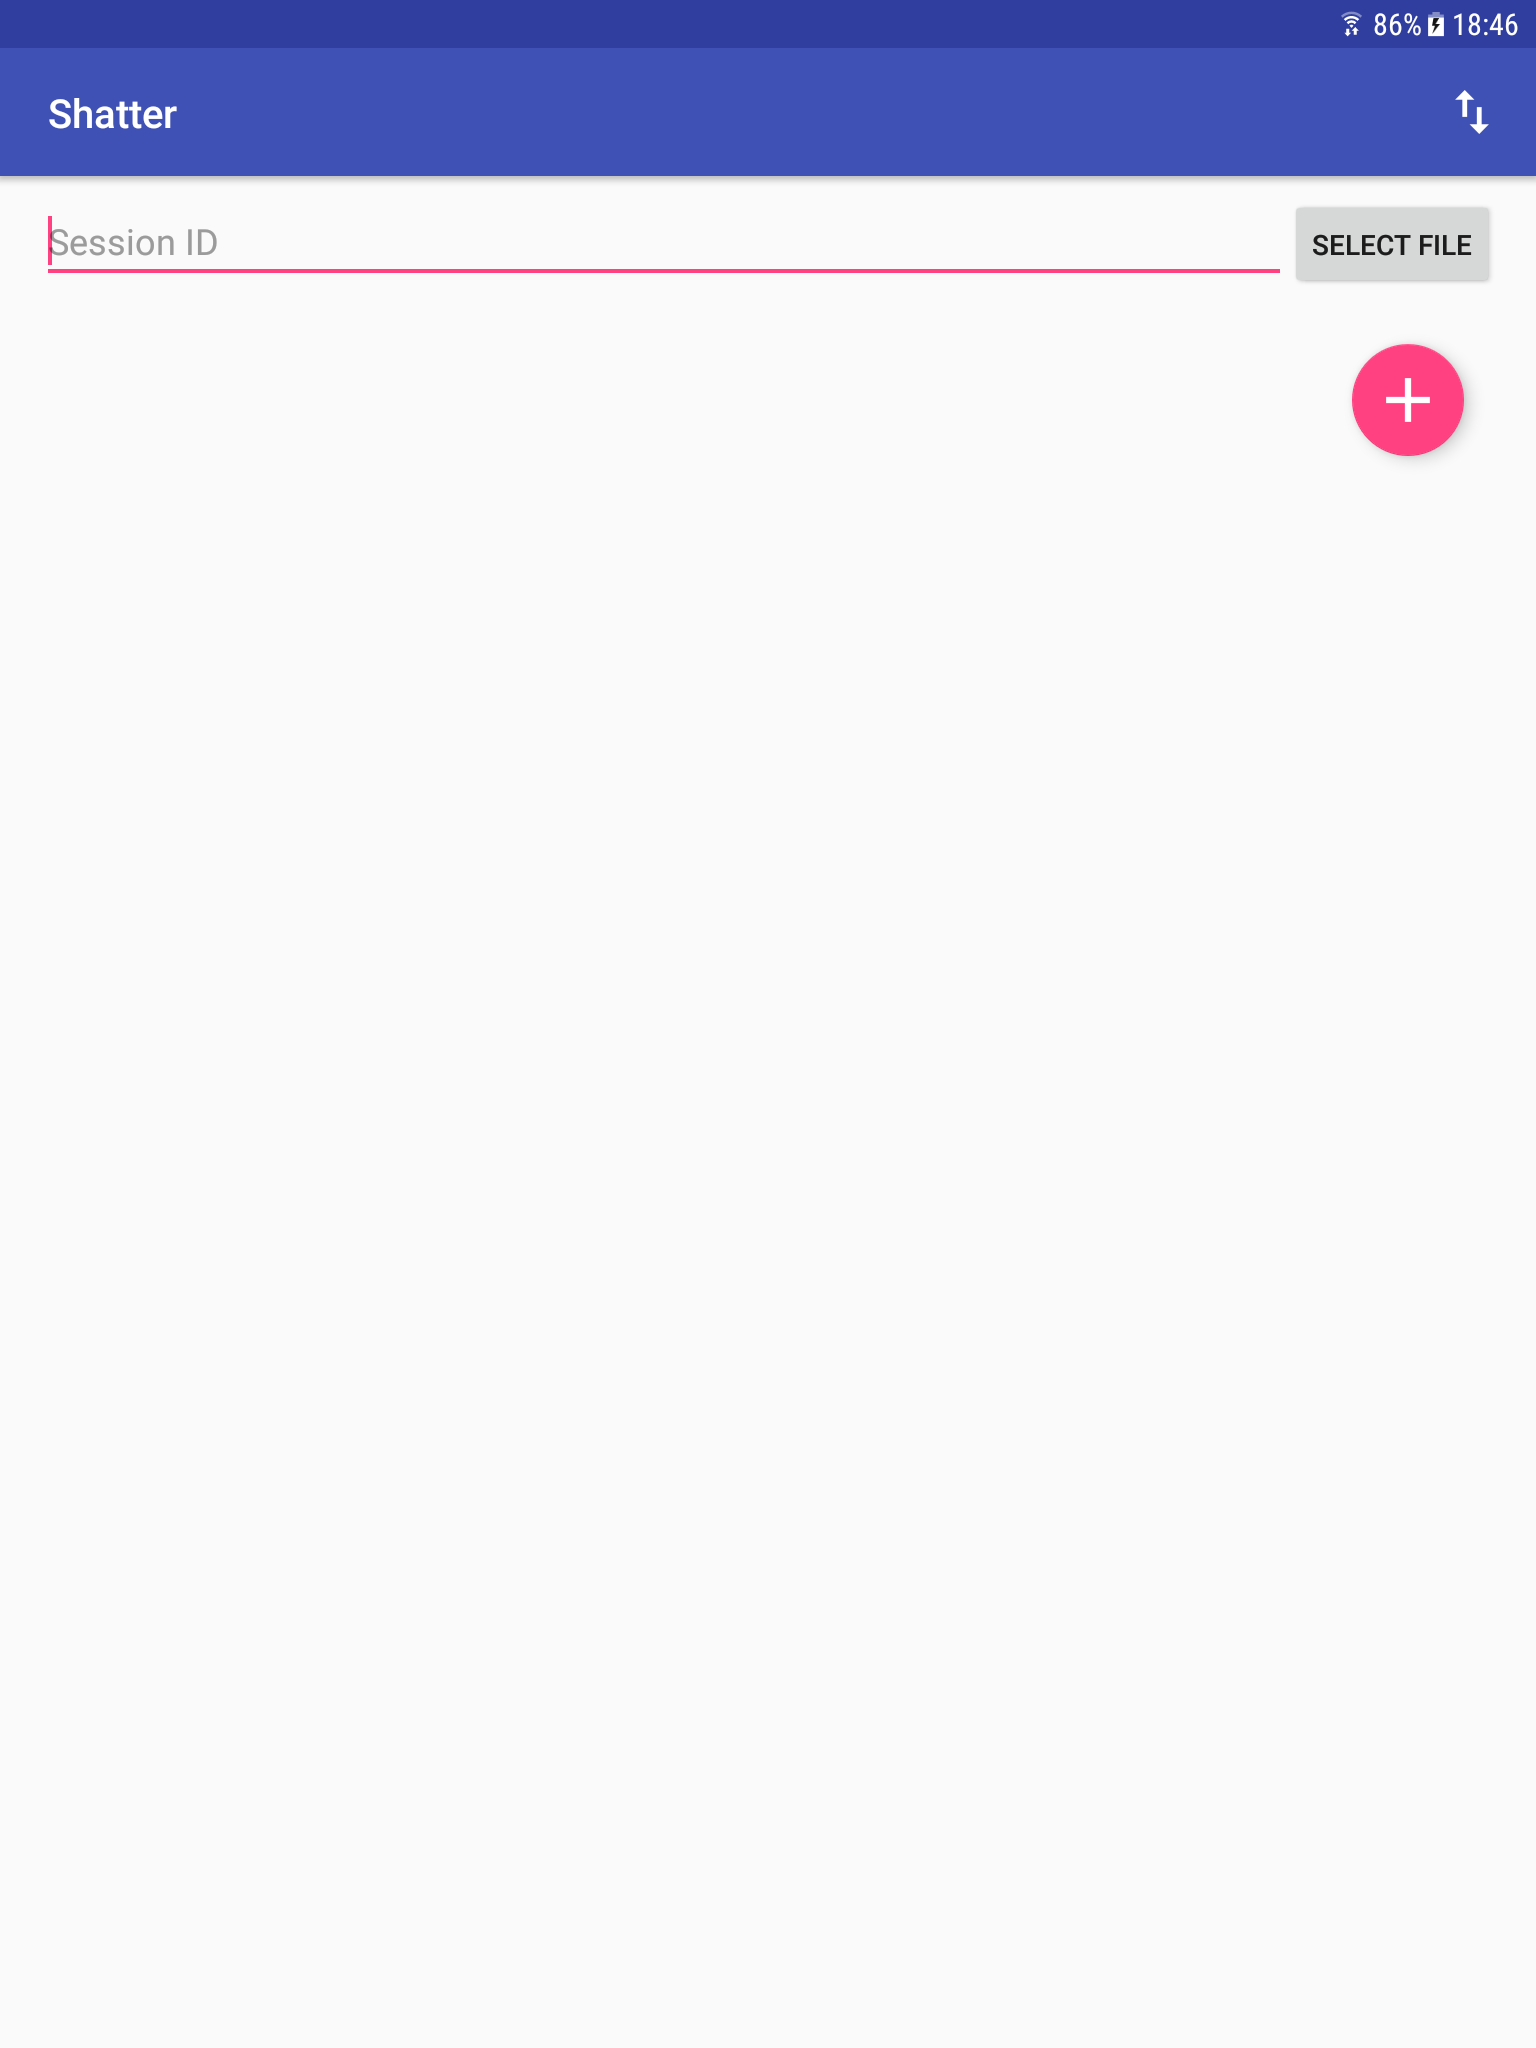
\includegraphics[scale=0.4]{Figures/home}
  \decoRule
  \caption[Shatter (Home)]{Pantalla principal de la aplicación}
  \label{fig:home}
\end{figure}

El primer objetivo es añadir algún usuario a la lista de contactos. Lo primero que hay que hacer es exportar la clave pública previamente generada haciendo uso del icono que se encuentra en la barra superior de la pantalla principal. (Figura~\ref{fig:export})

\begin{figure}[!htb]
  \centering
  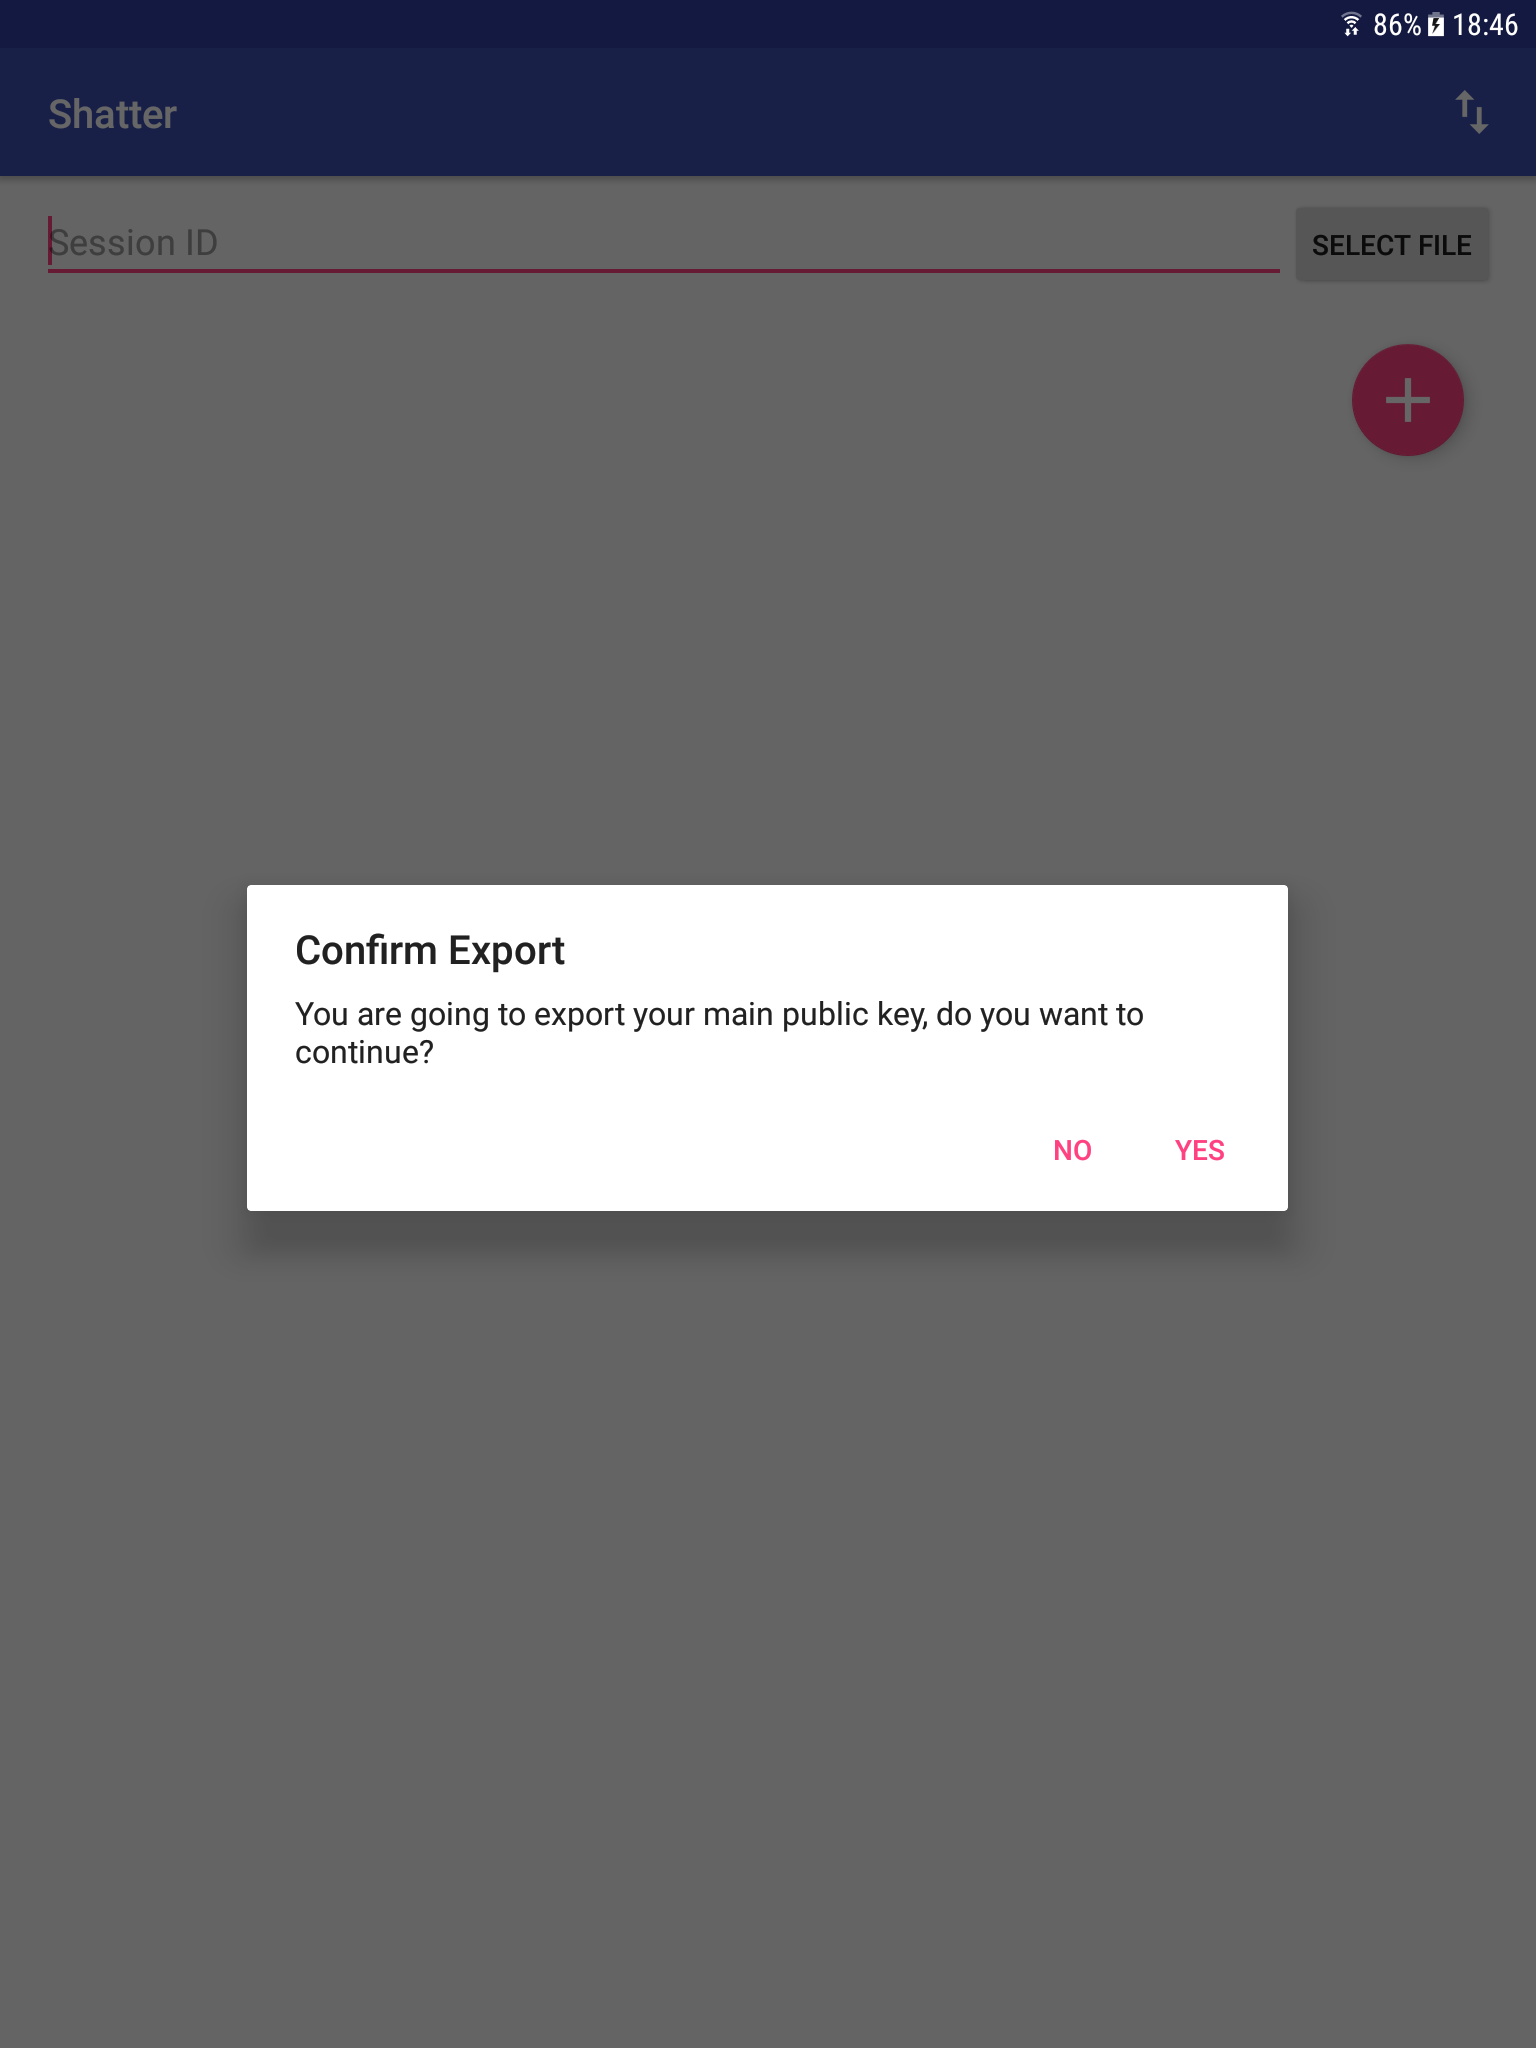
\includegraphics[scale=0.4]{Figures/export}
  \decoRule
  \caption[Shatter (Exportar clave pública)]{Mensaje de advertencia al exportar la clave pública}
  \label{fig:export}
\end{figure}

Al confirmar, se genera un certificado el cual contiene la clave pública antes generada en la ruta \path{Shatter/certs/main.crt}. \footnote{El directorio principal de la aplicación se encuentra en el almacenamiento externo del terminal y es accesible mediante un explorador de archivos.}

Para añadir a un contacto se dispone de un botón en la esquina inferior derecha de la pantalla principal, el cual abre una nueva pantalla en la que se puede especificar un alias (nombre de usuario) y un certificado con la clave pública del nuevo usuario. (Figura~\ref{fig:import})

\begin{figure}[!htb]
  \centering
  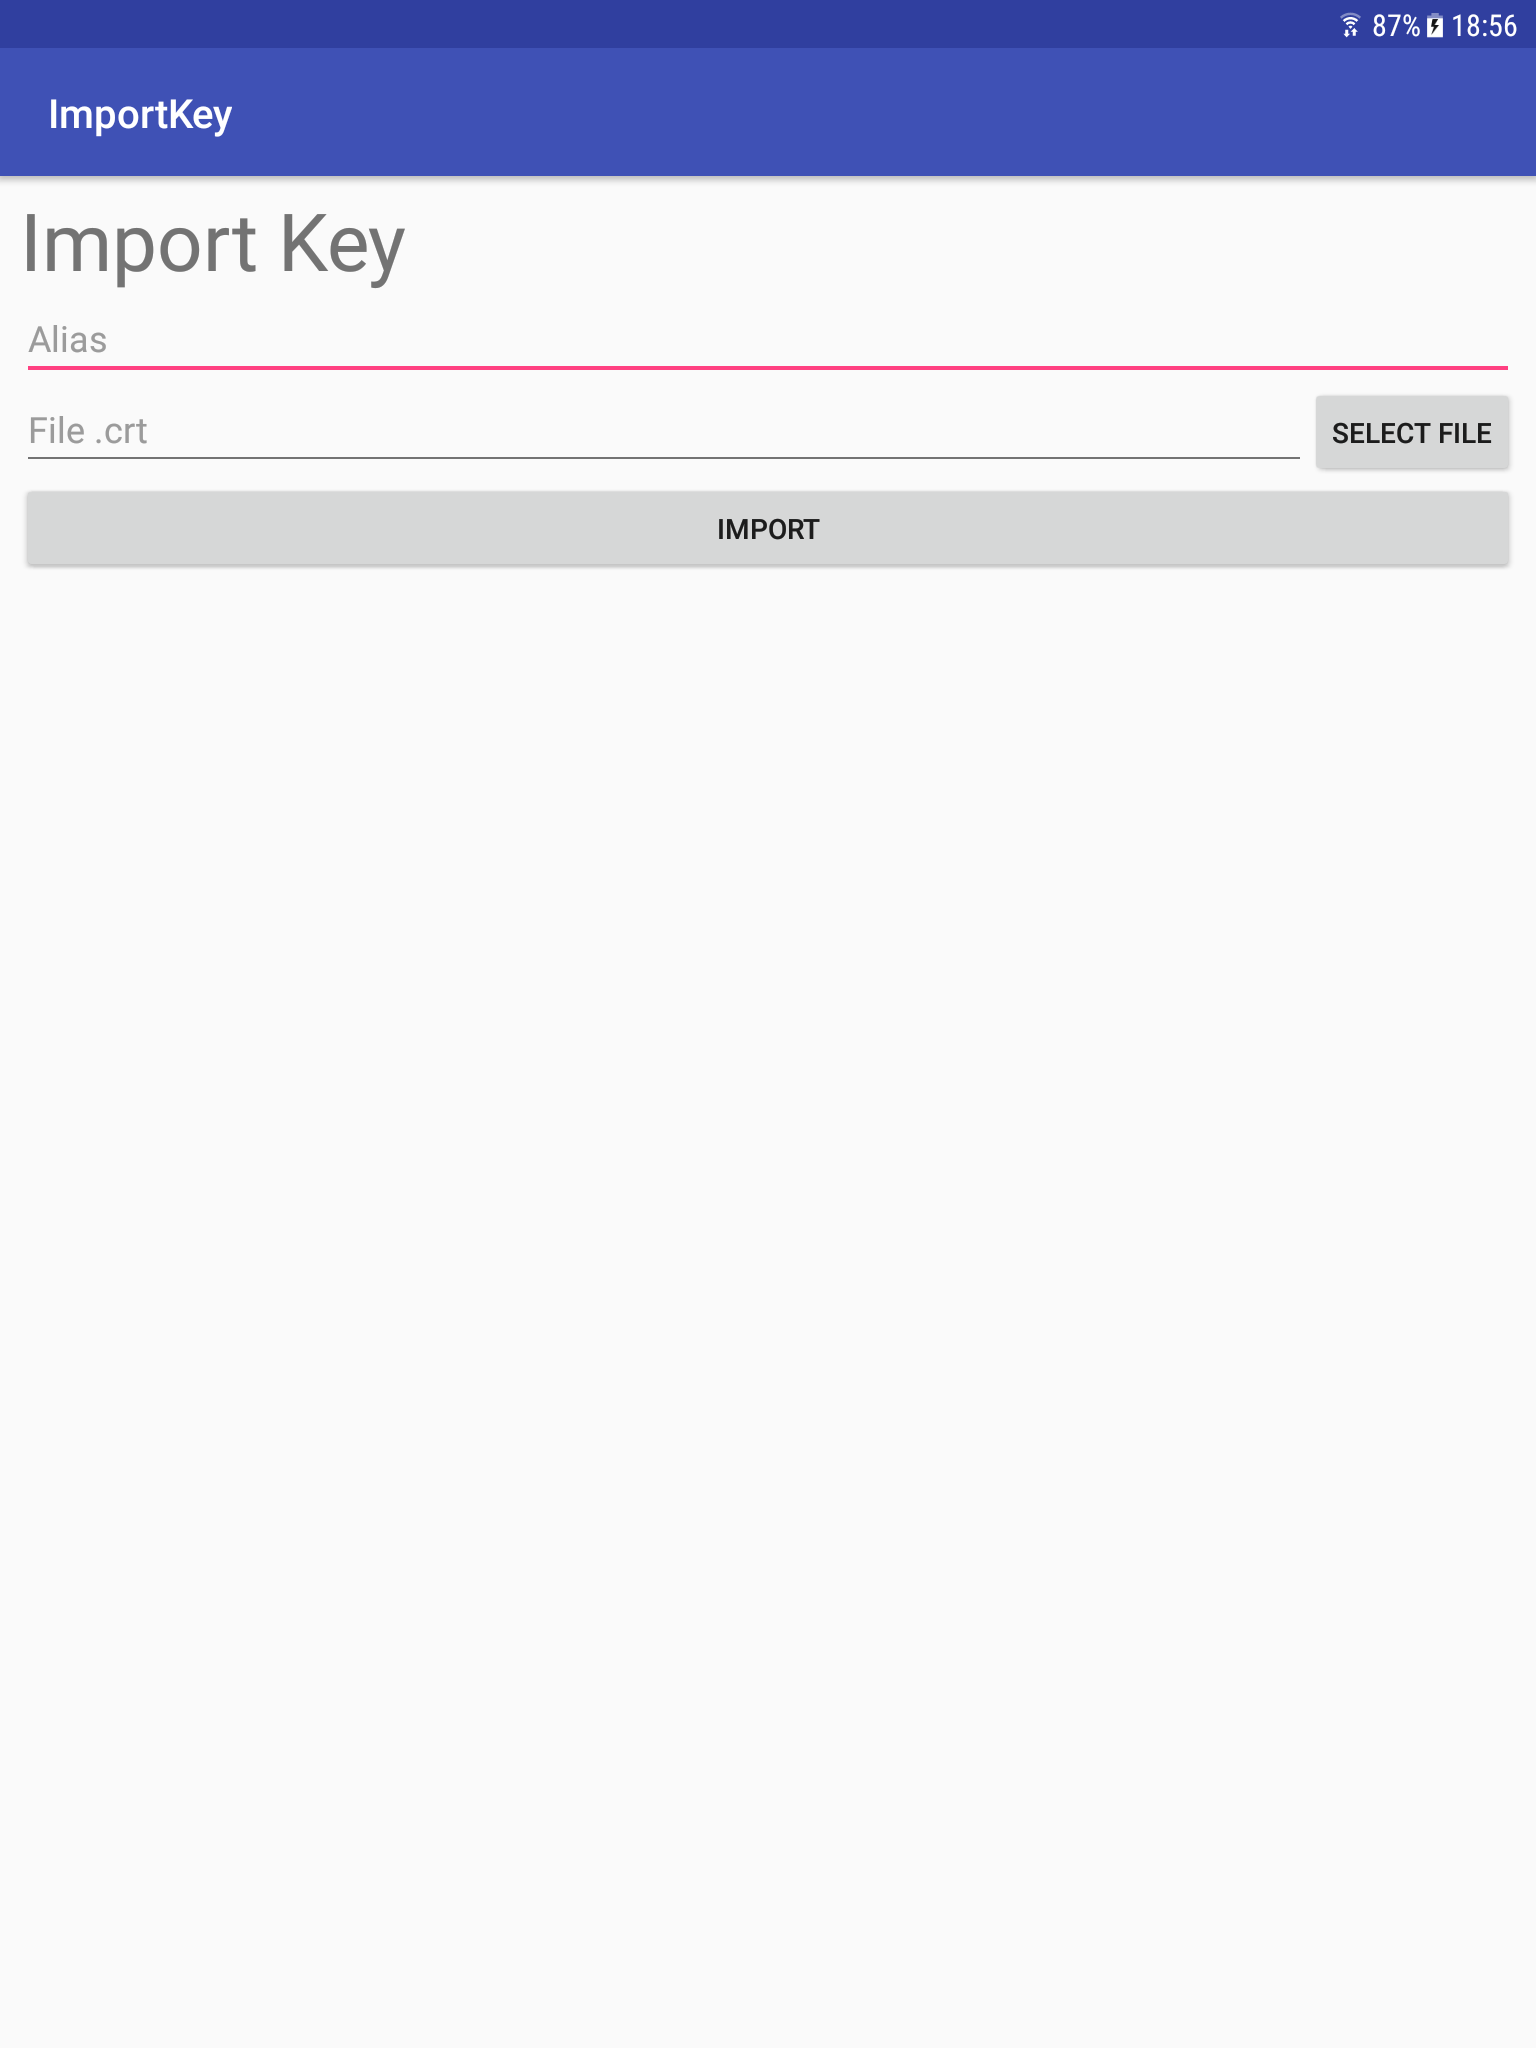
\includegraphics[scale=0.4]{Figures/import}
  \decoRule
  \caption[Shatter (Importar clave pública)]{Pantalla para importar la clave pública de un nuevo usuario}
  \label{fig:import}
\end{figure}

%De la misma manera, el nuevo contacto debe importar el certificado antes generado para poder llevar a cabo comunicaciones seguras.

Una vez el nuevo usuario se ha importado, la pantalla principal se actualiza y muestra el alias que tiene asignado, junto a unos botones con los que se puede operar con su clave pública. (Figura~\ref{fig:home_2})

\begin{figure}[!htb]
  \centering
  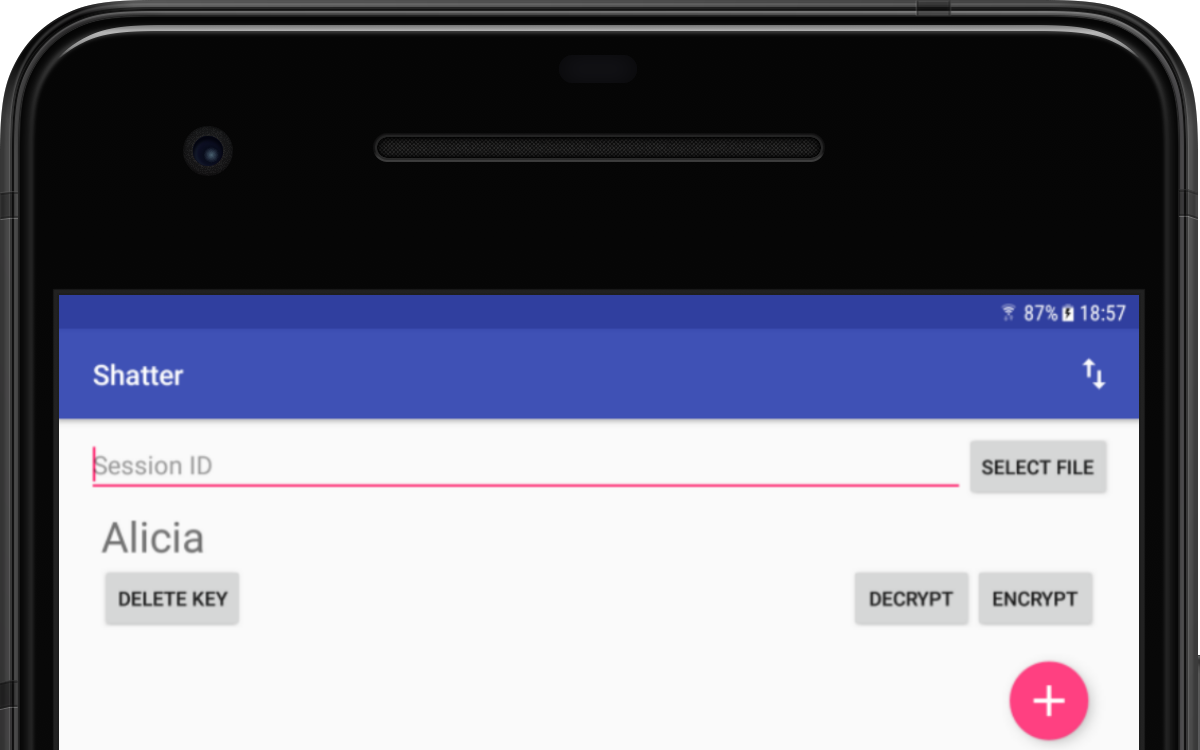
\includegraphics[scale=0.4]{Figures/home_2}
  \decoRule
  \caption[Shatter (Pantalla principal con usuarios)]{Pantalla principal de la aplicación con usuarios añadidos}
  \label{fig:home_2}
\end{figure}

\subsection{Cifrado y envío}

Para enviar un mensaje a un contacto, se debe utilizar el botón \keyword{\emph{Select File}}, el cual abre una nueva pantalla para elegir un fichero (Figura~\ref{fig:file_picker}). El selector de ficheros pone en el campo de texto de la pantalla principal el path absoluto del fichero seleccionado (también se puede escribir a mano), y ya solo queda tocar el botón \keyword{\emph{Encrypt}} del usuario al que vaya destinado el mensaje para que el fichero se fragmente y encripte. Si todo ha salido bien, se puede ver un mensaje en pantalla informando de ello, y en la ruta \path{Shatter/send/ID} se encuentran los fragmentos junto con la clave. (Figura~\ref{fig:encfiles})

\begin{figure}[!htb]
  \centering
  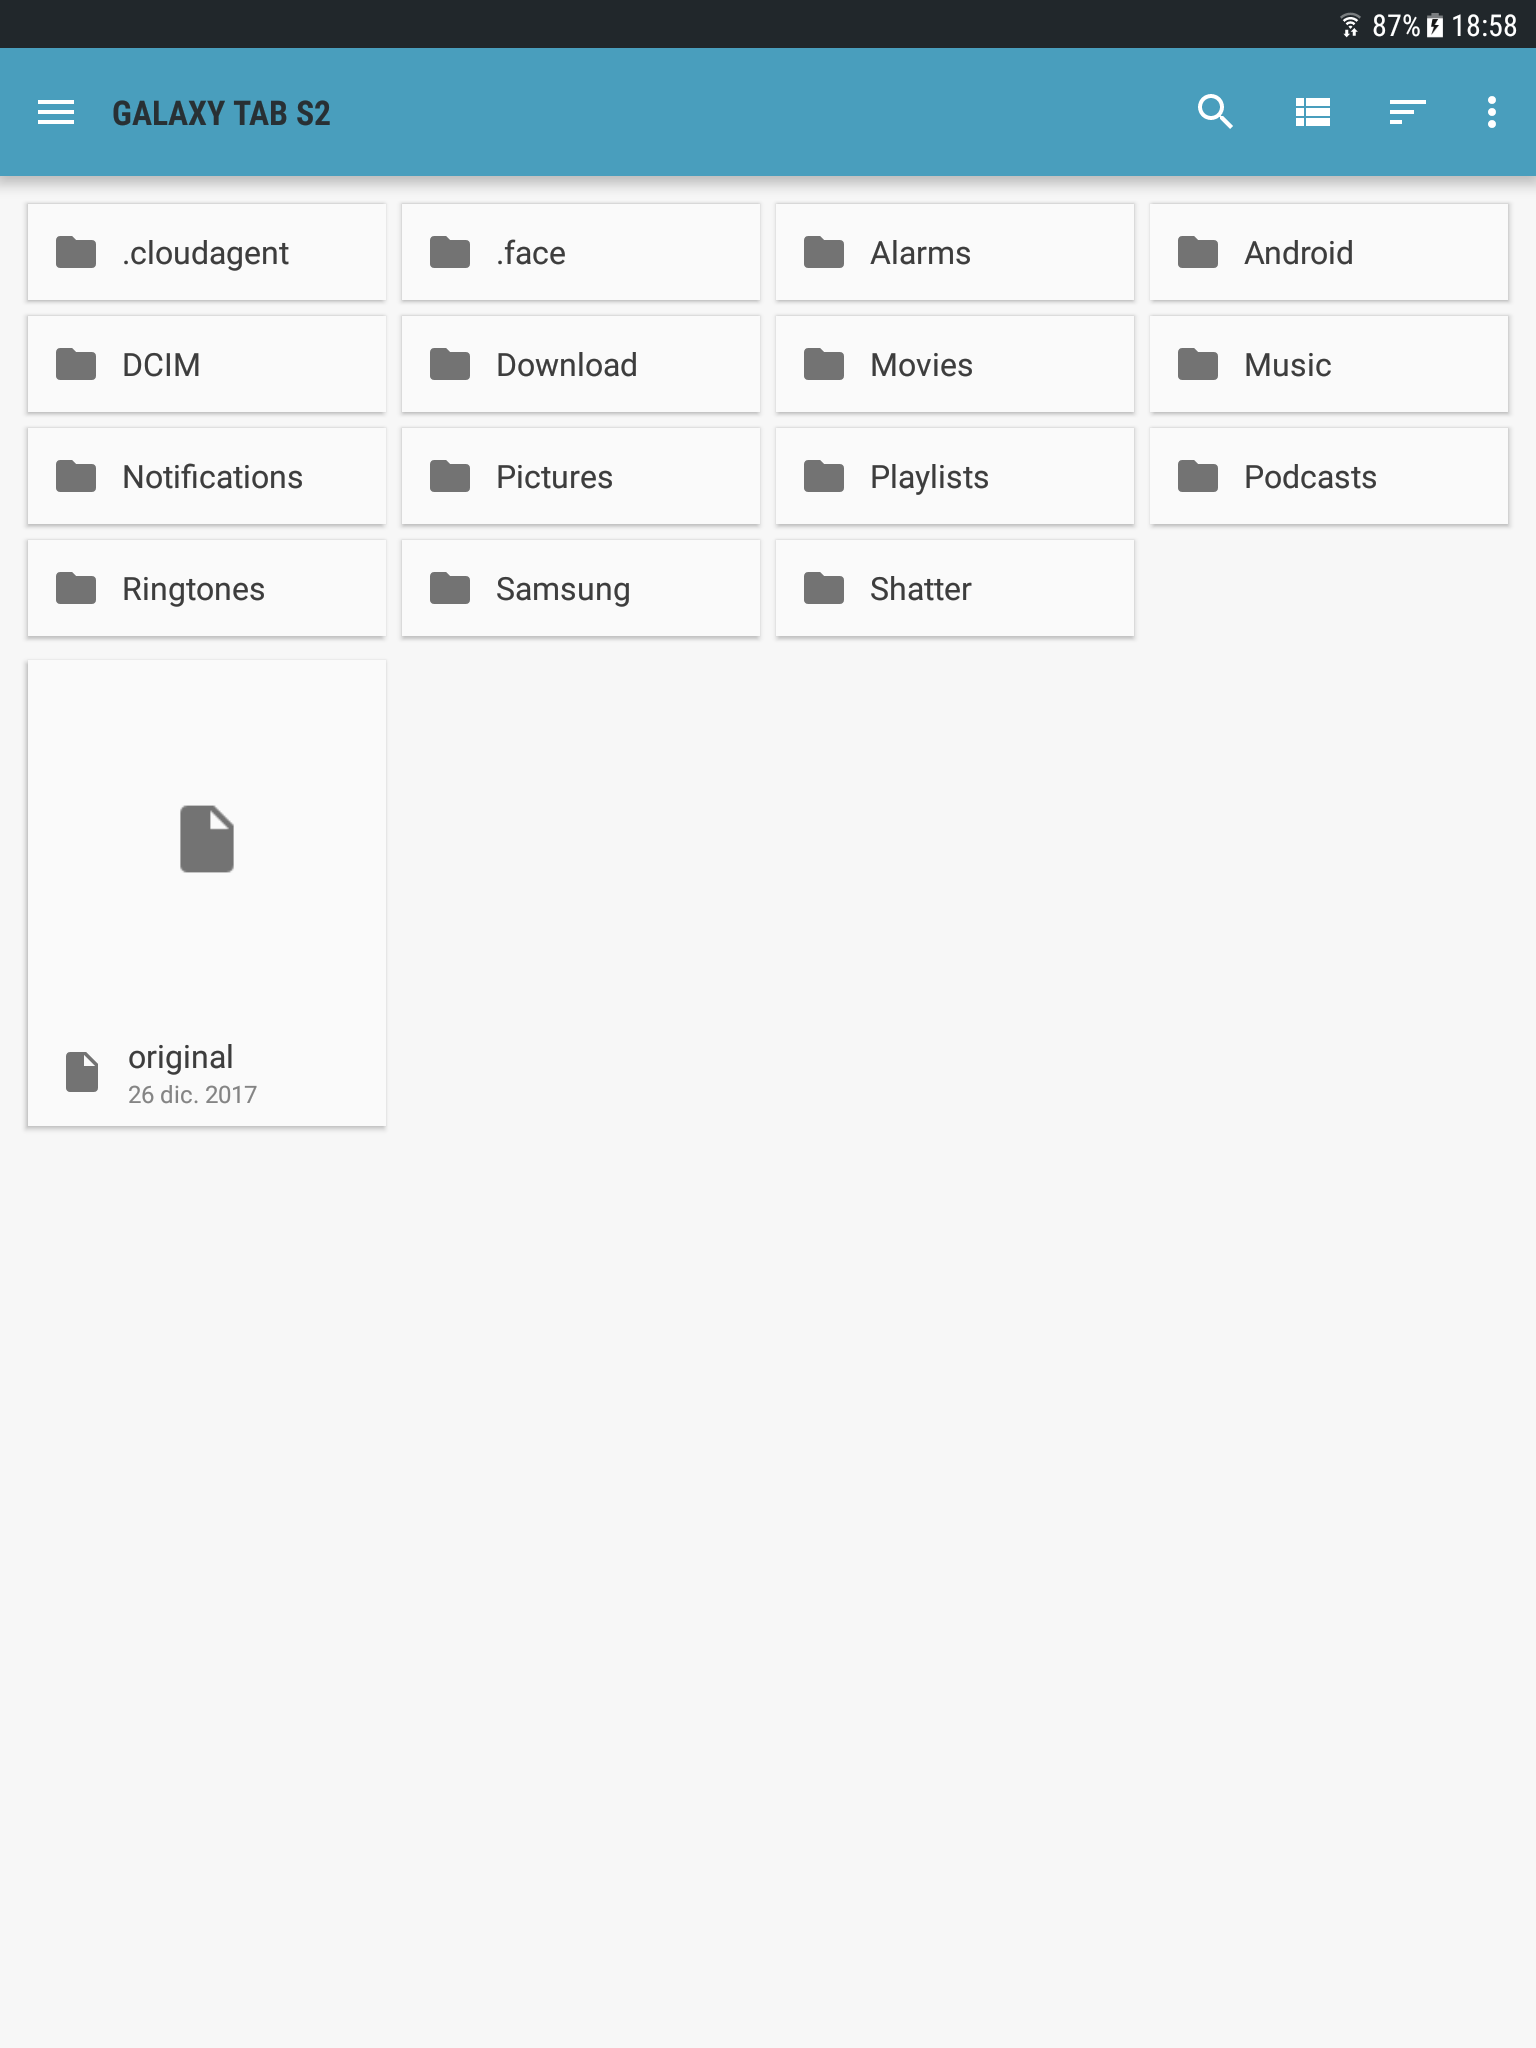
\includegraphics[scale=0.4]{Figures/file_picker}
  \decoRule
  \caption[Shatter (File Picker)]{Pantalla para seleccionar un fichero}
  \label{fig:file_picker}
\end{figure}

\begin{figure}[!htb]
  \centering
  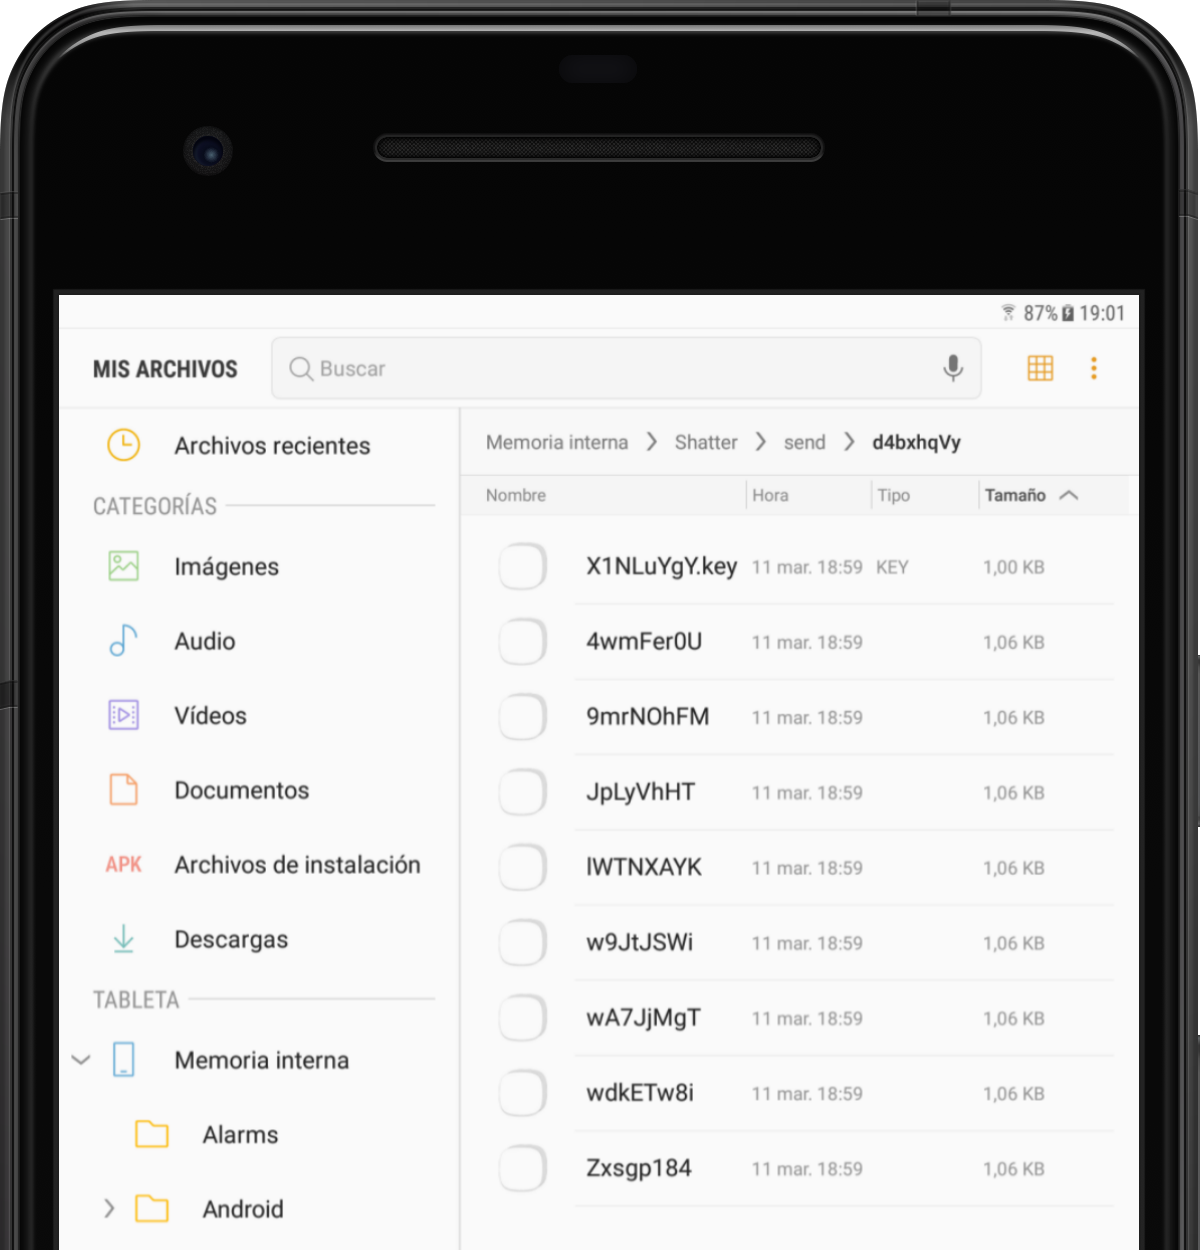
\includegraphics[scale=0.4]{Figures/encfiles}
  \decoRule
  \caption[Shatter (Mensaje fragmentado)]{Fragmentos de un mensaje junto a su clave}
  \label{fig:encfiles}
\end{figure}

El ID generado se debe comunicar al contacto al que vaya destinado, pero antes se debe subir el directorio que contiene los fragmentos al servidor haciendo uso del comando scp de Linux, por lo que se debe disponer de un usuario habilitado en la máquina que aloja el servidor. \footnote{En caso de estar encriptando el mismo mensaje para varios usuarios, se puede saber que ID corresponde a cada usuario mirando un registro que se encuentra en la ruta \path{Shatter/list.txt}}

\lstset{basicstyle=\ttfamily}
\begin{lstlisting}[language=bash]
  $ scp Shatter/send/ID server
\end{lstlisting}

\subsection{Descarga y descifrado}

Para descargar un mensaje de un contacto determinado, este debe comunicar de alguna manera el ID del mensaje, el cual se debe escribir en el campo de texto de la pantalla principal. A continuación se pulsa el botón \keyword{\emph{Decrypt}} asociado al alias del contacto.
%Si nuestro contacto quisiera descargarse el mensaje, escribirá el ID que le comunicamos antes en el campo de texto de la pantalla principal. Como sabe que el mensaje viene de nuestra parte, tocará el botón \emph{Decrypt} de nuestra clave pública.

Con esto, la aplicación pide al servidor un índice con todos los ficheros asociados a ese ID y descarga todos los que pueda en el directorio \path{Shatter/ID}. En caso de que algún fichero falte, informa de ello al usuario antes de proceder con el descifrado y rellena un registro indicando cuales son los fragmentos que faltan. (Figura~\ref{fig:miss})

\begin{figure}[!htb]
  \centering
  
\includegraphics[scale=0.4]{Figures/miss}
  \decoRule
  \caption[Shatter (Faltan fragmentos)]{Mensaje advirtiendo de que algunos fragmentos no se han descargado}
  \label{fig:miss}
\end{figure}

Si todos los fragmentos y la clave son descargados exitosamente, la aplicación procede con el descifrado de los mismos. Durante el proceso se crean, en caso de ser necesario, ficheros de registro en los cuales se reflejan los problemas surgidos. En caso de no ocurrir ningún problema, el fichero original se recompone en la ruta \path{Shatter/ID/done/ID}. (Figura~\ref{fig:done})

\begin{figure}[!htb]
  \centering
  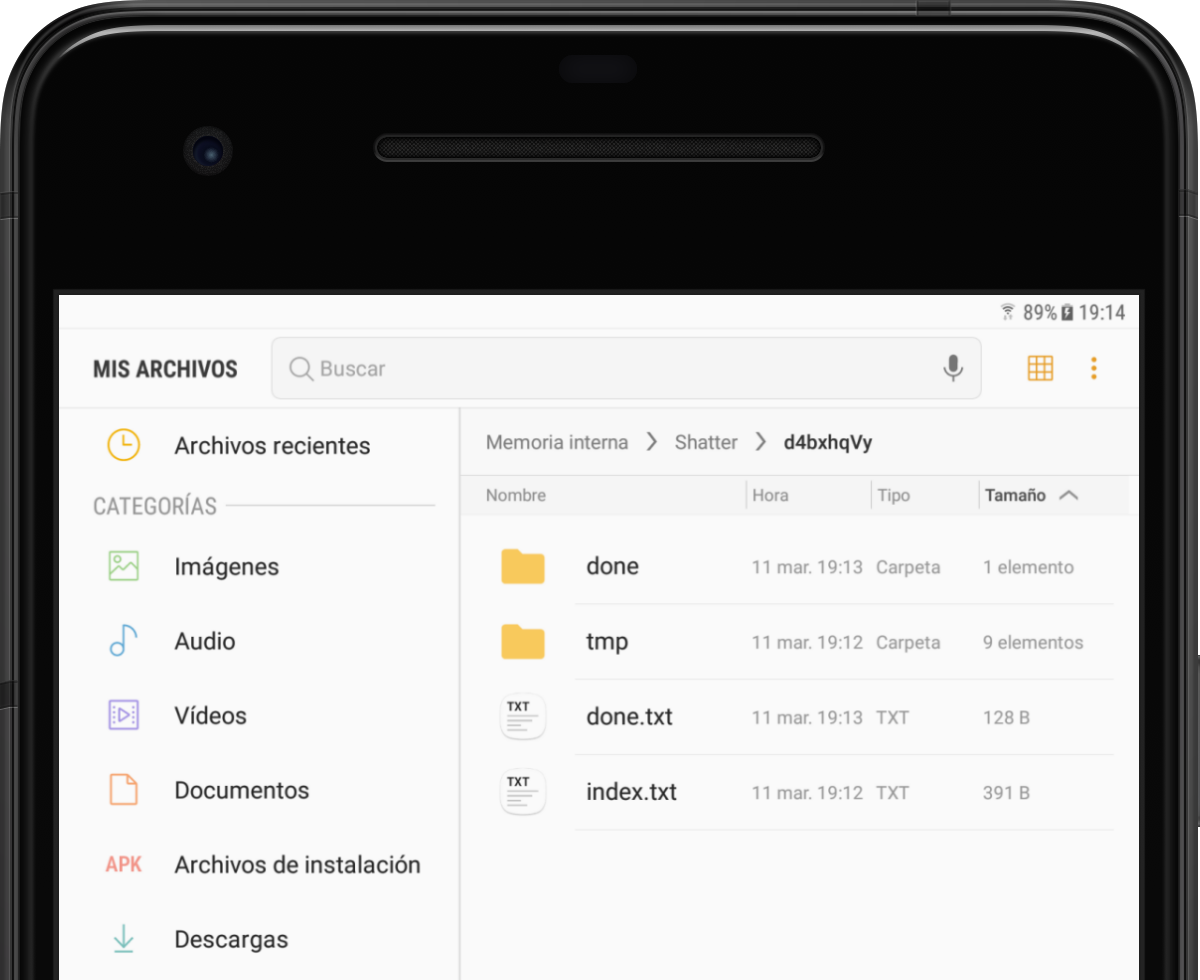
\includegraphics[scale=0.4]{Figures/done}
  \decoRule
  \caption[Shatter (Mensaje recibido)]{Directorio de un mensaje recibido}
  \label{fig:done}
\end{figure}

%-------------------------------------------------------------------------------

\section{Problemas encontrados}

A lo largo de la etapa que supuso el desarrollo de la aplicación, se han encontrado varios problemas que dificultaron la finalización del proyecto.

El mayor problema con el que se tuvo que lidiar es el no haber creado una parte portable que hiciera más fácil la migración a Android. Algunas librerías usadas cuando el proyecto solo era una aplicación escrita en Java tienen ciertas dependencias, las cuales no se encuentran en ninguna librería Java usada en Android. Además, el uso del Keystore de Android para almacenar las claves exige realizar el cifrado asimétrico, las firmas y la generación de las claves de una manera determinada, lo que supuso la eliminación de las clases que se encargaban anteriormente de ello (RSALibrary y RSAPSS). Aunque algunos de estos problemas no se habrían podido solucionar aun teniendo una parte portable, sin duda habría supuesto un ahorro considerable de tiempo.

A raíz de lo anterior, la mayoría de las clases no estuvieron bien definidas desde un principio. Esto supuso muchos cambios a lo largo del desarrollo de la aplicación (Cabeceras, modos de cifrado, registros...). De nuevo, una buena planificación habría ahorrado una gran cantidad de tiempo y energía.

Pero no todos los problemas encontrados tienen que ver con la desorganización. La aplicación ahora cuenta con un servidor dedicado pero, en un principio, se pensó en utilizar un servicio externo para el almacenamiento de los mensajes enviados por los usuarios. De algunas ideas que salieron, se eligió la aplicación Pastebin\footnote{\url{https://pastebin.com/}}, ya que permite la subida anónima de texto plano. La idea era que la aplicación subiera los distintos fragmentos cifrados a la plataforma, permitiendo al resto de usuarios su descarga. Sin embargo, la existencia de límites en el número de mensajes enviados o en la longitud de los mismos hicieron que se desechara la idea en favor de un servidor dedicado.

% Chapter 6: Last Conclusions

\chapter{Conclusiones finales} % Main chapter title

\label{Chapter6} % Reference

%----------------------------------------------------------------------------------------

\section{Objetivos alcanzados}

%----------------------------------------------------------------------------------------

\section{Líneas futuras}


%-------------------------------------------------------------------------------
%	THESIS CONTENT - APPENDICES
%-------------------------------------------------------------------------------

%\appendix % Cue to tell LaTeX that the following "chapters" are Appendices

% Include the appendices of the thesis as separate files from the Appendices folder
% Uncomment the lines as you write the Appendices

%% Appendix A

\chapter{Frequently Asked Questions} % Main appendix title

\label{AppendixA} % For referencing this appendix elsewhere, use \ref{AppendixA}

\section{How do I change the colors of links?}

The color of links can be changed to your liking using:

{\small\verb!\hypersetup{urlcolor=red}!}, or

{\small\verb!\hypersetup{citecolor=green}!}, or

{\small\verb!\hypersetup{allcolor=blue}!}.

\noindent If you want to completely hide the links, you can use:

{\small\verb!\hypersetup{allcolors=.}!}, or even better: 

{\small\verb!\hypersetup{hidelinks}!}.

\noindent If you want to have obvious links in the PDF but not the printed text, use:

{\small\verb!\hypersetup{colorlinks=false}!}.

%\include{Appendices/AppendixB}
%\include{Appendices/AppendixC}

%-------------------------------------------------------------------------------
%	THESIS CONTENT - CONCEPTS INDEX
%-------------------------------------------------------------------------------

\printindex

%-------------------------------------------------------------------------------
%	BIBLIOGRAPHY
%-------------------------------------------------------------------------------

\printbibliography[heading=bibintoc]

%-------------------------------------------------------------------------------

\end{document}
